% Fichero principal para libro de MATLAB y Octave para editorial Garceta
\documentclass[11pt, table]{book}

% -----------------------------------------------
% Título y autor
% -----------------------------------------------
\title{Introducción a la programación funcional}
\author{Santiago Higuera de Frutos \\ \vspace{1em}\small Universidad Politécnica de Madrid}
\date{ 
	\begin{center}
		
\includegraphics[width=0.3\textwidth]{img/Rustacean-orig-noshadow.png}
	\end{center}
%	\begin{center}
%		
\includegraphics[width=0.25\textwidth]{img/rust-logo.png}
%	\end{center}
   \begin{center}
      \footnotesize \textbf{\color{red}(Versión de fecha  \today)}
   \end{center}
}

% Fichero de estilo para este libro
\usepackage{../../garceta_2024}
\usepackage{../../codeboxes}



% -----------------------------------------------
% Inicio del documento
% -----------------------------------------------
\begin{document}
\lstset{language=Rust, style=colouredRust}

\pagestyle{empty}

\begin{center}
   
\includegraphics[width=\textwidth]{img/banner_ice.png}
\end{center}

{\centering \vspace{5em} \Huge\bfseries  Introducción a la programación funcional \par}

{\centering \vspace{5em} \Huge\bfseries  (Parte I) \par}

{\vspace{2em} \centering Santiago Higuera de Frutos \par}

{\centering \small Universidad Politécnica de Madrid \par}

\begin{center}
   
\includegraphics[width=0.3\textwidth]{img/Rustacean-orig-noshadow.png}
\end{center}
%	\begin{center}
   %		
\includegraphics[width=0.25\textwidth]{img/rust-logo.png}
   %	\end{center}
\begin{center}
   \footnotesize \textbf{\color{red}(Versión de fecha  \today)}
\end{center}


%\maketitle


\blankpage
%\pagestyle{fancy}
% -----------------------------------
% Dedicatoria
\pagestyle{empty}

\vfill
\begin{flushright}
\begin{minipage}{0.7\textwidth}
\begin{flushright}
\footnotesize
\textit{A los alumnos y profesores de la Universidad Politécnica de Madrid y al oficio de profesor, que tan pocos reconocimientos recibe, a pesar de su importancia en la creación de una sociedad mejor.} \\
\textbf{Santiago}
\end{flushright}
\end{minipage}
\end{flushright}

\blankpage


% -----------------------------------
% Tablas de contenidos
\dominitoc
\setcounter{tocdepth}{1} % Índice con secciones
\pagestyle{indice}
\renewcommand{\thepage}{\roman{page}}
\setcounter{page}{7}
{\small
	\tableofcontents
}
\vfill\null
\pagebreak

\blankpage
% ------------------------------------
% Prólogo
% ------------------------------------
\pagestyle{empty}
\chapter*{Prólogo}
\addstarredchapter{Prólogo}
\chaptermark{Prólogo}
\label{sec_prologo}

\noindent La programación funcional no es nueva. El lenguaje LISP (LISt Processing) está considerado uno de los primeros lenguajes de alto nivel que se desarrollaron, junto a Fortran y Cobol. Durante mucho tiempo se ha considerado un paradigma de programación demasiado teórico y alejado de la resolución de los problemas habituales en la programación real.

\smallskip

Durante ese tiempo, la Programación Orientada a Objetos (POO) se consideraba el paradigma base necesario para la programación en cualquier lenguaje. Con el tiempo, la POO ha mostrado algunas de sus debilidades, originadas por el mecanismo de la herencia entre tipos. Ya en 1994 ``\textit{The gang of four}'', en su famoso libro ``\textit{Design Patterns: Elements of Reusable Object-Oriented Software}'',  indicaban que había que primar la composición frente a la herencia al construir los programas \citep{gammaDesignPatternsElements1994}. 

\smallskip

En los últimos años, la programación funcional ha adquirido especial relevancia. Los principios que rigen la programación funcional son muy simples. Los principales lenguajes han ido incorporando algunos de los elementos que caracterizan a la programación funcional, como las funciones de orden superior, las closures, la inmutabilidad y otros. Es posible escribir programas con un estilo funcional casi en cualquier lenguaje.

\smallskip

Rust es un lenguaje de programación con solo unos años de vida pero que está teniendo un crecimiento muy importante debido la seguridad del manejo de memoria que proporciona, a la velocidad de ejecución del código generado, a la calidad de las herramientas que proporciona y a las buenas sensaciones que proporciona al programar. Rust no es un lenguaje funcional estricto, pero proporciona suficientes elementos para poder ser utilizado como tal. 

\smallskip

A lo largo del curso, se va a hacer una introducción a la utilización del lenguaje Rust y a los conceptos que sustentan el paradigma de la programación funcional. Se utilizará principalmente el lenguaje Rust, aunque también se mostrarán ejemplos en otros lenguajes.

\smallskip

Al final del curso, el alumno comprenderá los conceptos que subyacen bajo el paradigma de la programación funcional, de forma que podrá utilizar algunos de ellos en el lenguaje que utilice habitualmente. Ademas, conocerá los conceptos fundamentales de la programación con Rust, lo que le permitirá adentrarse en el lenguaje, si lo considera de interés.

%\blankpage

%\chapter*{Nota}
\addstarredchapter{Nota}
\chaptermark{Nota}
\label{sec_prologo}

\noindent Con el fin de optimizar el tiempo disponible, sería deseable que los alumnos instalaran en los ordenadores que vayan a utilizar en el curso, el entorno de desarrollo de Rust.

\smallskip

El entorno de desarrollo consta del lenguaje Rust y de un editor de texto.

\smallskip

Se adjunta el capítulo 2 de la documentación del curso, en el cual se explica cómo hacerlo.


%\blankpage


\vfill\null
\pagebreak

% -----------------------------------
% Acerca de los autores
\thispagestyle{vacio}
{\centering \huge\textbf{Acerca del autor}\par}
\vspace{6em}

\begin{minipage}{0.9\textwidth}
	\setlength{\parindent}{0pt}
	
	{\centering\large\textbf{Santiago Higuera de Frutos} \par}
	\vspace{1em}
	
	\begin{wrapfigure}{l}{0.4\textwidth} 
		\centering\vspace{-0.5\baselineskip}
		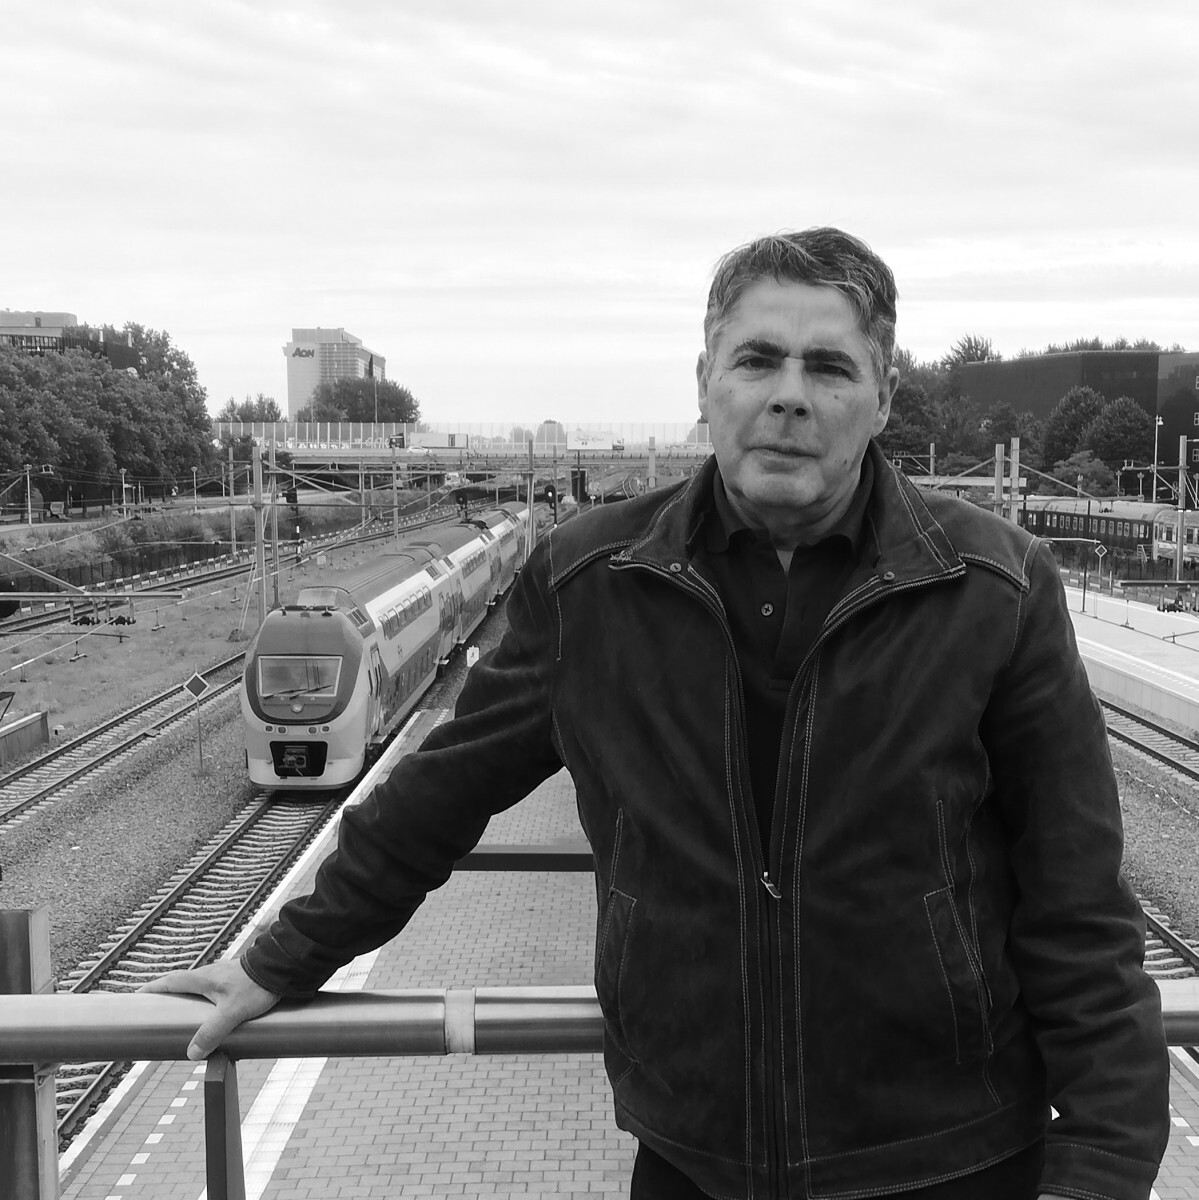
\includegraphics[width=0.4\textwidth]{img/FotoSantiago_bw.jpg}
	\end{wrapfigure}
	
	Doctor Ingeniero de Caminos por la Universidad Politécnica de Madrid (UPM). Ha sido profesor en la Escuela de Ingenieros de Caminos y actualmente en Teleco Campus Sur. Es autor de los libros ``\textit{Programacion en Rust}'' y  ``Programación y métodos numéricos para Ingeniería con MATLAB y Octave'', publicados por la Editorial Garceta, así como de numerosos artículos y conferencias sobre programación, geometría de las carreteras y simuladores de conducción, todo ello en el ámbito del software de código abierto. 
\end{minipage}

\blankpage

\cftpagenumbersoff{section} % Suprime los números de página en las minitablas de contenido generadas con el paquete minitoc. Debido a las interacciones entre tocloft y minitoc, hay que hacerlo desde aquí y no funciona la orden de minitoc \mtcsetpagenumbers{minitoc}{off}. Además, hay que dar la orden después de haber generado el \tableofcontents

\setcounter{minitocdepth}{1} % Índices de los capítulos solo con secciones
% ------------------------------------

% ------------------------------------
% Capítulos
% ------------------------------------
\pagestyle{fancy}
\renewcommand{\thepage}{\arabic{page}}
\setcounter{page}{1}

% Contenido del CursoICE_2024
\chapter{Pensar de manera funcional. Programación declarativa}
\label{ch_intro}

\IndiceCapitulo
\begin{Resumen}
   Se considera que la programación funcional está basada en el \textit{cálculo lambda},  un sistema formal desarrollado en los años 1930 para investigar la naturaleza de las funciones, de la computabilidad y su relación con la recursión. 
   
   \smallskip
   
   El objetivo de este curso es explicar las técnicas y la forma funcional de razonar en programación para mejorar la calidad del código de los programas.
\end{Resumen}

\section{¿En qué consiste la programación funcional?}
Es difícil definir el concepto de \textit{Programación Funcional} (PF). Se considera que la PF está incluida en el paradigma de la \textit{programación declarativa}, en la cual los lenguajes se centran en describir qué quieren hacer en lugar de detallar cómo hacerlo, como sucede en los lenguajes imperativos.

Los siguientes elementos formarían parte del conjunto de componentes que utilizan los lenguajes funcionales:

\begin{itemize}
   \item \textbf{Funciones puras:} se dice que una función es \textit{pura} si no produce efectos secundarios, no depende de ningún estado exterior y siempre proporciona el mismo resultado para el mismo valor de los argumentos de entrada. Se entiende por \textit{efecto secundario} cualquier acción del programa que no sea un cálculo. Por ejemplo, modificar el estado de una variable, mostrar un mensaje en una pantalla o enviar un correo electrónico serían ejemplos de efectos secundarios.
   \item \textbf{Funciones de orden superior:} las funciones que operan utilizando otras funciones se denominan \textit{funciones de orden superior}. En la programación funcional, las funciones se consideran \textit{elementos de primera clase}, lo que significa que se pueden tratar como cualquier otro tipo de datos: se pueden utilizar como parámetros o como valor devuelto por otras funciones y pueden asignarse a variables. En la mayoría de lenguajes hay elementos que no son de primera clase, por ejemplo los operadores o las cláusulas que definen los bucles o las bifurcaciones.
   \item \textbf{Closures:} en programación funcional es habitual utilizar un tipo especial de funciones denominadas \textit{closures}. Se trata de funciones anónimas definidas in situ que son capaces de capturar el entorno en el que fueron definidas, de forma que pueden acceder con posterioridad a variables de ese entorno con los valores que tuvieran en el momento en el que se declaró la \textit{closure}. Actualmente, las \textit{closures} también se incluyen en numerosos lenguajes, a veces bajo la denominación de \textit{funciones anónimas}.
   \item \textbf{Inmutabilidad de las variables:} la programación funcional pone especial énfasis en la utilización de estructuras \textit{inmutables}. Cambiar el valor de una variable, cambiar su estado, se considera un efecto secundario que hay que tratar de evitar. Decir que las \textit{variables} no deben variar puede parecer un contrasentido, pero no es un asunto excepcional en los lenguajes de programación. Por poner un ejemplo, en Java o en Javascript, las variables del tipo \textit{String} son inmutables. Cuando se quiere modificar el estado de una variable inmutable lo que se hace es crear una nueva variable con el nuevo valor. El procedimiento consiste en \textit{transformar} una variable en otra, en vez de en modificar el estado de la variable original. La inmutabilidad facilita los test de los programas y hace más segura la utilización de la programación multiproceso o en paralelo.
   \item \textbf{Recursividad:} el control de flujo en la programación funcional favorece la recursividad frente a los bucles. Sustituyendo los bucles del tipo \textit{for} o \textit{while} mediante recursividad se consigue un código más declarativo y, en ocasiones, más elegante.
   \item \textbf{Iteradores:} los \textit{iteradores} son una construcción habitual en la programación funcional y que, a día de hoy, incorporan muchos lenguajes. Son estructuras que permiten recorrer una colección de manera ordenada, sin recurrir a bucles y variables de índice. 
   \item \textbf{Evaluación perezosa:} las expresiones, siempre que se pueda, se deben comportar de manera \textit{perezosa}. La \textit{evaluación perezosa} (\textit{lazy evaluation}) consiste en que determinados cálculos que impliquen a variables no se realicen hasta que son estrictamente necesarios.
   \item \textbf{Sin estado ni efectos secundarios:} en la programación funcional se trata de minimizar los estados mutables y los efectos secundarios. El resultado es un código en el que es más fácil razonar, hacer test y realizar la depuración de errores. Cuando es necesario mantener estados o realizar acciones con efectos secundarios, se controla rigurosamente.
\end{itemize}

Tras leer los párrafos anteriores, el lector puede estar preguntándose cómo es posible realizar un programa de aplicación práctica sin efectos secundarios y sin cambiar el valor de las variables. Bien, no es posible, los programadores funcionales utilizan funciones impuras en numerosas ocasiones y necesitan utilizar variables mutables en determinados contextos. No obstante, durante el desarrollo de un programa, hay numerosas situaciones en las que la utilización de funciones puras y el respeto a la inmutabilidad proporciona más seguridad y da lugar a que el código generado sea más escalable.

La programación funcional no es una sintaxis determinada, consiste en una serie de técnicas orientadas a eliminar los efectos secundarios o, al menos, limitar su alcance. Si se utilizan estas técnicas de manera adecuada, se consigue escribir código más fácil de leer, más correcto, más seguro, más fácil de probar y más fácil de depurar, lo que a fin de cuentas es el objetivo fundamental que se debe perseguir al programar. 

La técnicas de la programación funcional no están restringidas por el lenguaje de programación que se utilice. Los conceptos que se utilizan en la programación funcional se pueden aplicar a la programación orientada a objetos o a la programación basada en procedimientos. Son principios generales que producen beneficios en la codificación de cualquier programa y en cualquier lenguaje. En realidad se trata de buenas prácticas de codificación de carácter universal.

\section{Diferencias con la Programación Orientada a Objetos}
A partir de los años 90 del siglo pasado, la Programación Orientada a Objetos (POO) se convirtió en el paradigma fundamental de programación. Si no sabías programar orientado a objetos, no sabías programar. Se enseñaba de una forma muy dogmática e incluso se suponía que había que \textit{pensar orientado a objetos}. Cualquier programa se tenía que razonar en términos de clases y objetos, en lo que se denominaba \textit{análisis y diseño orientado a objetos}.

A medida que se fueron desarrollando programas con esta metodología, se comprobó que la POO daba lugar a ciertos desarrollos que producían programas con código complicado, difícil de comprender y que además dificultaba la depuración y la realización de test. Se comprobó que la POO se adaptaba mejor a cierto tipo de problemas que a otros.

El mundo real no siempre se puede modelizar bien haciendo una descomposición en categorías con propiedades bien definidas. Por ejemplo, se puede organizar una jerarquía para el reino animal que divida los animales en mamíferos, reptiles, aves, etc. Y cuando ya está organizada, aparece el ornitorrinco, que no encaja correctamente en ninguna de las categorías que se habían previsto\footnote{\textit{``The platypus effect'' (el efecto ornitorrinco)} es un término acuñado por Anselm Hook y del que yo he tenido conocimiento a través del artículo ``\textit{The Rise and Fall of Object Oriented Programming}'' de David ``Talin'' Joiner.}. La solución puede ser crear una nueva categoría para el ornitorrinco o rehacer la jerarquía de clases para darle cabida. Cualquiera de las dos soluciones es muy costosa en términos de esfuerzo y complejidad.

Es frecuente que las jerarquías de clases sean muy profundas, con muchos niveles de clases que van heredando unas de otras. Las clases en lo alto de la jerarquía tienen métodos y propiedades que solo utilizan unas pocas clases, así como métodos para mantener estados que en muy rara ocasión se modifican. 

\pagebreak
A menudo, esta complejidad está originada por tratar de poner juntas cosas que nada tienen en común. Por ejemplo, si se están modelizando figuras, se tienen figuras como la esfera o el cubo. Pero si además se quiere dar cabida a esferas rojas o azules, cubos rojos o azules, etc, se podría caer en crear categorías específicas para las esferas rojas, las esferas azules, los cubos rojos y los cubos azules. Erich Gamma et al., la \textit{banda de los cuatro} (\textit{the Gang Of Four, GoF}), ya indicaron en 1994 en su libro ``Design Patterns''  \citep{gammaDesignPatternsElements1994}, que había favorecer la composición frente a la herencia. En la parte izquierda de la Figura \ref{fig_herencia_composicion} se puede ver la jerarquía de clases que se obtendría priorizando el mecanismo de herencia. En la parte derecha de la misma figura se puede ver el resultado cuando se aplica la composición. 

\begin{figure}[htb]
   \begin{center}
      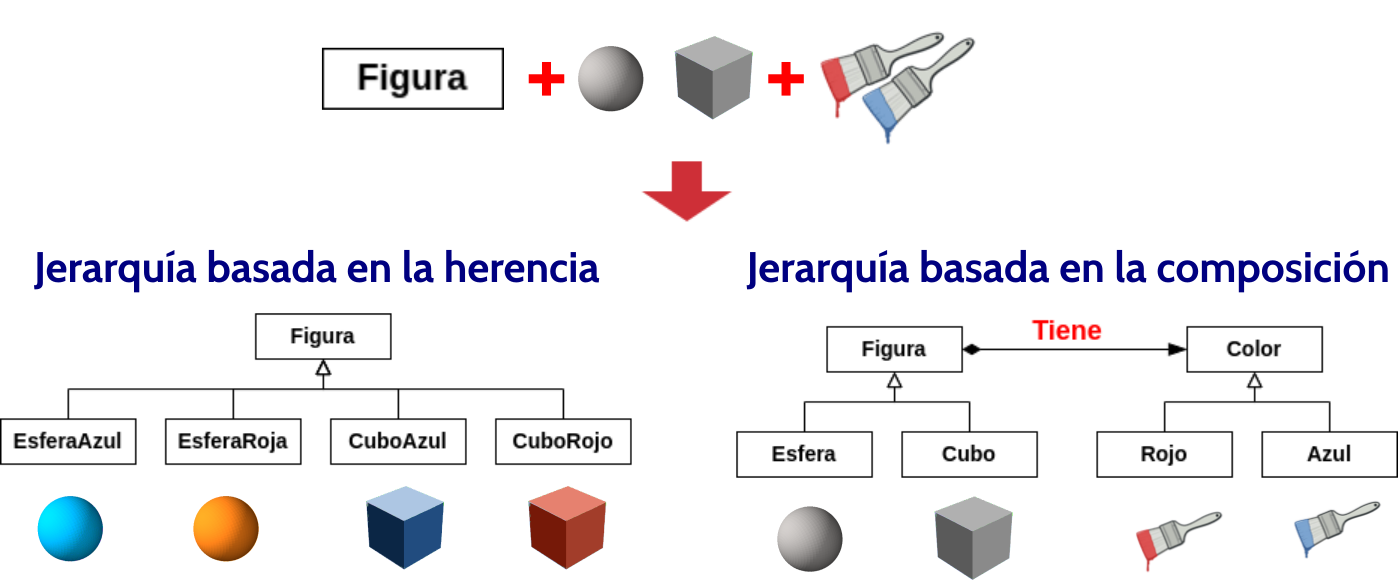
\includegraphics[width=\textwidth]{img/herencia_composicion.png}
      \caption{Diferentes jerarquías de clases según se priorice la herencia o la composición.}
      \label{fig_herencia_composicion}
   \end{center}
\end{figure}

En general, la composición da lugar a jerarquías de clases menos intrincadas, más sencillas de comprender y que se adaptan mejor a las pruebas, la depuración y las modificaciones.

Modelar el mundo a base de clases y objetos no deja de ser un tema subjetivo: cada programador puede encontrar diferentes formas de entender la jerarquía de categorías necesaria. De hecho, cada entidad de la vida real (\textit{clase}) puede servir para cosas muy diferentes (métodos de la clase). Por ejemplo, una taza puede servir para \textit{beber()}, pero también podría servir como arma (\textit{lanzar()}) o como \textit{pisapapeles()}.

Una de las reglas que se considera que debe cumplir cualquier diseño orientado a objetos es la \textit{encapsulación}, según la cual, el estado de los objetos no se debe poder modificar directamente desde fuera del objeto, sino solo a través de los métodos que proporciona la clase en cuestión. 

Por ejemplo, si se tuviera una clase denominada \textit{Etiqueta} con una propiedad llamada \textit{texto}, no se debería poder borrar el texto de la etiqueta mediante una instrucción del tipo:

{\centering \texttt{etiqueta.text = `` '';} \par}

Un diseño correcto proporcionaría un método \textit{borrar()} que realizase dicha acción de borrar el texto de la etiqueta:

{\centering \texttt{etiqueta.borrar();} \par}

Este procedimiento funciona perfectamente cuando las operaciones son sencillas, pero la cosa se complica cuando las acciones a realizar implican varios objetos de distintas clases. En esos casos, puede ser más sencillo utilizar funciones ajenas a las propias clases. Es una cuestión casi semántica: ¿en qué debemos poner más énfasis, en los sustantivos (\textit{Etiqueta}) o en los verbos (borrar()).

A medida que las jerarquías de clases crecen se hace cada vez más difícil preparar test que permitan probar los nuevos métodos que se implementan. Cada nuevo método necesita mucho trabajo de preparación para los test, y esta complejidad se incrementa de manera exponencial a medida que crece la jerarquía de clases.

Un planteamiento alternativo es que las clases prácticamente solo tengan datos y que las funciones que se necesiten para operar sobre esos datos sean externas a las clases. Esta técnica da lugar a una organización del código mucho más sencilla. Cada función solo realiza una tarea y cuando se quieren hacer test, solo hay que crear algunos juegos de datos de prueba y probar la función concreta, sin tener que luchar con una gran colección de clases y ficheros. Un caso típico donde este planteamiento es muy útil es cuando se trabaja con bases de datos relacionales, que se adaptan mal a la modelización de la POO.

Es ahí donde entran en juego las técnicas que proporciona la Programación Funcional (PF). Mientras que la Programación Orientada a Objetos se centra en la interacción y la comunicación entre diferentes objetos, la programación funcional se centra en cómo se van transformando los objetos. 

Dicha transformación hay que entenderla en el sentido de que un objeto se le pasa como argumento a una función que devuelve un nuevo objeto que incorpora las transformación que se quieren realizar. El objeto que devuelve la función es un nuevo objeto y el objeto original se puede conservar o desechar. En la programación funcional, unos objetos se transforman en otros, no se modifican.

\vfill\null

Se resumen a continuación algunas de las características de la programación orientada a objetos (POO):
\begin{itemize}
   \item \textbf{Estado de los objetos:} la POO está basada en objetos que encapsulan en una sola entidad su estado (propiedades) y su comportamiento (métodos). La \textit{mutabilidad} es una parte inherente de la POO. El estado de los objetos puede variar a lo largo del tiempo, lo que se consigue a través de los métodos que proporcionan las clases. De esta manera, se modelizan las entidades reales y sus relaciones. Esta mutabilidad es una forma natural de representar las propiedades de los objetos que necesitan cambiar de valor a lo largo del tiempo, pero da lugar a problemas complejos para gestionar estados globales y secundarios, por ejemplo en la programación concurrente.
   \item \textbf{Clases y herencia entre tipos:} la POO se basa en el concepto de clases como modelos de los objetos y a menudo utiliza la herencia entre clases para compartir y ampliar el comportamiento de las mismas.
   \item \textbf{Polimorfismo:} objetos de diferentes clases pueden ser tratados como si fueran de una misma clase base de la cual todos derivan.
   \item \textbf{Paradigma imperativo:} en general, la POO utiliza código con un paradigma imperativo, describiendo los pasos que hay que dar para modificar el estado de los objetos.
\end{itemize}

En el caso de la programación funcional (PF), algunas características distintivas son:
\begin{itemize}
   \item \textbf{Funciones sin estado:} está basada en la utilización de funciones que no mantienen ningún estado y operan sobre datos inmutables. En ese sentido, la PF separa el estado de los objetos de su comportamiento. El estado se representa mediante estructuras de datos inmutables. El comportamiento se expresa a través de funciones que operan sobre dichos datos.
   \item \textbf{Funciones como objetos de primera clase:} las funciones son objetos de primera clase que se pueden utilizar como parámetros de otras funciones, se pueden devolver como resultados y se pueden asignar a variables. Las funciones se utilizan para modelizar abstracciones, encapsular comportamientos. Para conseguir procesamientos complejos se utiliza la composición de funciones.
   \item \textbf{Paradigma declarativo:} la PF utiliza una codificación más declarativa, expresando la lógica de lo qué se quiere hacer, sin describir el flujo de instrucciones para ello. 
\end{itemize}

La opinión del autor es que no hay que ser fundamentalista de ningún paradigma de programación. Hay que recordar el viejo dicho: ``\textit{al que la única herramienta que conoce es el martillo, todo le parecen clavos}''. Hay problemas que se adaptan mejor a unas técnicas de programación u otras. En muchas ocasiones, una combinación adecuada de las técnicas de la POO y de la PF será lo más adecuado. En todos los casos hay que analizar el problema que se trata de resolver y utilizar la combinación de técnicas que mejor se adapte al mismo.


% ---------------------------------------------------
\chapter{``¡Hola, Mundo!'' en Rust}
\label{ch_hola_mundo}
% ---------------------------------------------------
\IndiceCapitulo

\begin{Resumen}
Para poder seguir el contenido del curso es importante tener instalado el entorno de desarrollo del lenguaje Rust. La instalación es sencilla y rápida, si se siguen las instrucciones que se dan en la propia página del proyecto y que se indicarán en este primer capítulo de la documentación del curso. 

\smallskip

Además, es importante utilizar un editor de texto con los complementos necesarios para trabajar con Rust. Los contenidos del curso se han desarrollado utilizando Visual Studio Code de Micrososft y RustRover de Jet Brians. Ambos son editores de gran calidad y que ofrecen importantes ayudas a la programación en Rust.

\smallskip

Esté capítulo de la documentación del curso se completa con la explicación de cómo desarrollar el clásico programa ``¡Hola, Mundo!'' y con la explicación de algunos conceptos comunes, como la inclusión de comentarios en el código, la utilización de algunas macros del lenguaje útiles en entornos de depuración y pruebas y la posible utilización del portal ``Rust Playground''.
\end{Resumen}

\section{Instalación de Rust}

Para instalar el entorno de desarrollo de Rust, el método más sencillo es descargarse el \textit{script} de instalación que se proporciona para cada sistema operativo y ejecutarlo en el ordenador. Las instrucciones se dan en la página Web de Rust, en la siguiente dirección:

{\centering \small \texttt{https://www.rust-lang.org/tools/install} \par}

Los usuarios de Linux y de Mac no tendrán problema en seguir las instrucciones que se dan en dicha página. Los usuarios de Windows pueden descargar el instalador directamente del siguiente enlace:

{\centering \footnotesize \texttt{https://static.rust-lang.org/rustup/dist/i686-pc-windows-gnu/rustup-init.exe} \par}

Para poder compilar y construir los programas se necesita un \textit{linker}. Es posible que ya lo tenga instalado en su sistema. Si aparecieran errores relativos a la falta del \textit{linker}, hay que instalar un compilador de \texttt{C}, que suele tener el \textit{linker} ya incorporado. En cualquier caso, es útil tener un compilador de \texttt{C} instalado en el sistema, pues algunos paquetes pueden depender de él para su correcto funcionamiento.

Los usuarios de \textit{Linux} pueden instalar \texttt{GCC} o \texttt{Clang}, el que sea acorde a su distribución. Los usuarios de \textit{Ubuntu} pueden instalar el paquete \texttt{build-essentials}.

Los usuarios de \textit{macOS} pueden obtener un compilador de \texttt{C}
tecleando la siguiente instrucción:

{\centering \texttt{xcode-select --install}\par}

Los usuarios de \textit{Windows} deben seguir las instrucciones de instalación que se dan en la página web del proyecto Rust \citep{klabnikRustProgrammingLanguage}, en la siguiente dirección web:

{\centering\fontfamily{lmss}\selectfont{https://www.rust-lang.org/tools/install}\par}

Durante la instalación, se le indicará al usuario que necesita tener instaladas las herramientas de \texttt{C++} para \textit{Visual Studio 2013} o posterior. Se pueden instalar las herramientas para \textit{Visual Studio 2019} comprobando que se activa la opción correspondiente a la instalación de las \textit{C++ build tools}, el \textit{SDK} para \textit{Windows 10} y los componentes en inglés de dicho \textit{pack}.

La instalación que hace \texttt{rustup} incluye el programa \texttt{rustup}, el compilador \texttt{rustc} y el gestor de paquetes \textit{Cargo}. Para comprobar que el conjunto de desarrollo está correctamente instalado en el ordenador, se pueden probar las siguientes ordenes en la consola:

\begin{Codigo}
rustup show
rustc --version
cargo --version
\end{Codigo}

El resultado debería ser similar al de la Figura \ref{fig_rustup}.

\begin{figure}[H]
   \begin{center}
      \setlength\fboxsep{2pt}
      \setlength\fboxrule{0.5pt}
      \fbox{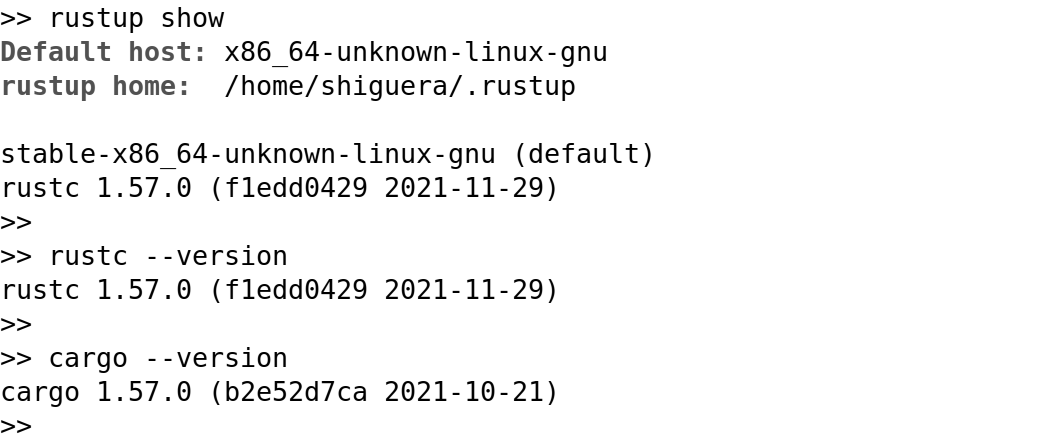
\includegraphics[width=0.9\textwidth]{img/figura_rustup_bw.png}}
      \caption{Instrucciones en el terminal para comprobar las versiones instaladas de los programas \textit{rustup}, \textit{rustc} y \textit{cargo}}
      \label{fig_rustup}
   \end{center}
\end{figure}

Si no aparecen los mensajes y se está trabajando en \textit{Windows}, debería comprobar que Rust está en la variable \texttt{\%PATH\%} del sistema. En adelante, las instrucciones que se indican en este libro deberían de funcionar en los terminales de cualquiera de los tres sistemas operativos.

Para actualizar a una versión más reciente de Rust, hay que teclear en el terminal la siguiente instrucción:

{\centering\texttt{rustup update}\par}

Para desinstalar Rust hay que teclear:

{\centering\texttt{rustup self uninstall}\par}

Al instalar Rust, se carga en el ordenador una versión de la documentación. Mediante la siguiente instrucción, se puede consultar dicha documentación localmente en el navegador:

{\centering\texttt{rustup doc}\par}

Podrá navegar a través de multitud de documentos y libros que le servirán para profundizar sobre Rust. En particular, un buen comienzo es el ``Libro de Rust'', escrito y mantenido por Steve Klabnik y Carol Nichols, con contribuciones de la \textit{Rust Community}. Además de la copia que se instala en su ordenador, puede consultar la versión más actualizada en la web, en la referencia \citep{klabnikRustProgrammingLanguage}:

{\centering \small \texttt{https://doc.rust-lang.org/book/} \par}

El portal oficial de Rust ofrece enlaces a diversos documentos de interés en la siguiente dirección:

{\centering \small \texttt{https://www.rust-lang.org/learn} \par}

Cuando le surjan dudas acerca de alguna función o instrucción de las que se explican en este libro, la mejor manera de acceder a una documentación más completa de la misma es la referencia de la API de la librería estándar. La documentación local le ofrecerá una copia, o también la puede 
consultar en la web en la referencia \citep{rustfoundationRustStandardLibrary}.

A día de hoy, existen numerosos libros donde iniciarse o profundizar en los distintos aspectos del lenguaje. Como no podía ser de otra manera, el autor de estas líneas considera que su libro ``Programación en Rust'', publicado en la Editorial Garceta, es una buena herramienta para aprender a programar en Rust \citep{higueradefrutosProgramacionRust2022}.

Otras editoriales que disponen de libros sobre Rust son:
\begin{itemize}
   \item \textit{Packt}: {\small \texttt{https://www.packtpub.com/}}
   \item \textit{Manning}: {\small \texttt{https://www.manning.com/}}
   \item \textit{O'Reilly}: {\small \texttt{https://www.oreilly.com/}}
\end{itemize}

\subsection{El editor de texto}

\noindent Para completar el entorno de trabajo, será necesario disponer de un editor. El código de los programas en lenguaje Rust se escribe en ficheros de texto plano. Se puede utilizar cualquier editor de texto para ello. En el siguiente enlace se muestran los editores que están comprobados por la fundación Rust y que proporcionan herramientas de compilación integradas, ayudas y corrección de sintaxis y otras:

{\centering \small \texttt{https://www.rust-lang.org/tools} \par}

El autor utiliza habitualmente Visual Studio Code de Microsoft y RustRover de JetBrains. 

\textit{Visual Studio Code} de \textit{Microsoft} \citep{VisualStudioCode}, es una buena opción. Hay versiones para cualquier sistema operativo, es gratuito, de buena calidad y dispone de una buena integración con Rust. El nombre con el que se suele denominar al
programa es \textit{VS Code}.

Para sacar el máximo provecho de la utilización de \textit{VS Code} al programar en Rust, es conveniente instalar la extensión existente para Rust, que ofrece numerosas ayudas, como autocompletado, remarcado de errores, terminal para ejecutar las órdenes de compilación\footnote{En la opción del menú \texttt{View::Terminal}, el programa  \textit{VS Code} ofrece un terminal para ejecutar todos los comandos. En el caso de los usuarios de \textit{Windows}, el terminal ofrecido es \textit{Power Shell}, aunque se puede configurar para utilizar el terminal \texttt{cmd} estándar.}, gestión de paquetes
y otras utilidades que facilitan mucho la gestión de los programas en Rust. Se puede consultar cómo hacerlo en:

{\centering \small \texttt{https://code.visualstudio.com/docs/languages/rust} \par}

\textit{RustRover} está desarrollado por JetBrains. JetBrains dispone de editores de gran calidad para varios lenguajes. Son de pago, pero ofrece versiones completas de manera gratuita para estudiantes y profesores. Utilizando una cuenta de correo de la UPM, se puede disfrutar de dichas ventajas en todos los editores de JetBrains. El editor RustRover se puede desacargar desde la siguiente dirección:

{\centering \small \texttt{https://www.jetbrains.com/rust/} \par}

Los dos editores comentados son de gran calidad y también lo serán, con seguridad, el resto de editores recomendados por la Fundación Rust, aunque el autor no ha tenido ocasión de probarlos.

\pagebreak

\section{¡Hola, mundo! en Rust}
\noindent Siguiendo la tradición, se va a explicar cómo crear el primer programa en Rust, un programa que imprima \texttt{¡Hola, mundo!} en el terminal del ordenador. Se supone que se está trabajando en el terminal del sistema. Se recomienda crear un directorio para los programas escritos en Rust y, dentro de él, directorios individuales para cada programa. Para este primer programa, la forma de proceder en \textit{Linux, macOS} o \textit{Windows} con \textit{Power Shell} podría ser la siguiente:
\begin{Codigo}
mkdir ~/rust_projets
cd ~/rust_projects
mkdir hola_mundo
cd hola_mundo
\end{Codigo}

En el caso de estar trabajando en la terminal \texttt{cmd} de \textit{Windows}, las instrucciones equivalentes serían las siguientes:
\begin{Codigo}
mkdir "%USERPROFILE%\rust_projects"
cd /d "%USERPROFILE%\rust_projects"
mkdir hola_mundo
cd hola_mundo
\end{Codigo}

Con ello, se ha creado un directorio llamado \texttt{rust\_projects} en el directorio del usuario y, dentro de él, un directorio llamado \texttt{hola\_mundo}. Tras crear los directorios, nos hemos posicionado dentro del directorio \texttt{hola\_mundo}. Obsérvese que, para el nombre de los directorios del proyecto, se ha utilizado lo que será el convenio habitual para nombrar programas, variables y funciones en el lenguaje Rust, el denominado \textit{snake case}: letras minúsculas separando las palabras con el guión bajo.

A continuación, utilizando el editor de texto, cree un fichero llamado \texttt{main.rs} para teclear el código del programa. Los ficheros de código en Rust tienen la extensión \texttt{rs}. Se podría llamar al fichero con otro nombre, pero también es convenio que el programa que contiene la función \texttt{main()} se llame \texttt{main.rs}. Esta función  es lo primero que se ejecuta en los programas escritos en Rust. Teclee el siguiente código en la función recién creada:

\begin{Codigo}
fn main() {
   println!("¡Hola, mundo!");
}
\end{Codigo}

La primera línea es la signatura\footnote{En teoría de programación, se denomina \textit{signatura} de una función a la primera línea, en la que se declara el nombre, los parámetros y el valor devuelto por la función.} de la función \textit{main()}. Como se puede observar, consta de la palabra clave \textit{fn},
que indica al compilador que se está declarando una función, seguida por el nombre de la función, en este caso \textit{main}. A continuación se escriben dos paréntesis, en esta ocasión vacíos. Dentro de estos paréntesis se escriben los parámetros que admite la función. En este caso, la función \textit{main()} no recibe ningún parámetro. A continuación, se pondría el tipo de datos del valor devuelto por la función, pero en este caso la función \textit{main()} tampoco devuelve ningún valor.

A continuación se escribe el código de la función, encerrado entre una pareja de llaves \texttt{\{\}}. El convenio de escritura en Rust es escribir la llave de apertura en la línea de signatura; las instrucciones que componen el cuerpo de la función se escriben en las lineas siguientes, tabuladas hacia la derecha; finalmente, la llave de cierre de la función se escribe en una línea nueva tras la última instrucción, alineada con la palabra \texttt{fn} de la signatura.

Al instalar Rust, se instala también la utilidad \texttt{rustfmt} que permite formatear los ficheros de código fuente siguiendo los convenios de escritura de Rust. Para ello, solo hay que teclear en el terminal la orden siguiente:

{\centering\texttt{rustfmt nombre\_del\_fichero\_fuente}\par}

El código de la función \texttt{main()} recién creada consta de una sola línea. Se trata de la macro \texttt{println!()} que escribe una línea de texto en la pantalla. En este caso se le ordena escribir la cadena de caracteres \texttt{"¡Hola, mundo!"}. Se hablará algo más de la macro \texttt{println!()} en el Apartado \ref{sec_codigo_ejemplos}.

Para poder ejecutar el programa hay que compilarlo. Esto se consigue tecleando la siguiente instrucción en el terminal:

\vspace{0.2em}
{\centering\texttt{rustc main.rs}\par}

El programa \texttt{rustc} es el compilador de Rust. Al ejecutar la instrucción anterior, se compila el programa y se crea un ejecutable, llamado \texttt{main}. 

\pagebreak

Si tras esa instrucción se listan los ficheros del directorio, se ve que hay un fichero ejecutable \texttt{main}. En \textit{Windows}, el ejecutable se llama \texttt{main.exe} y además, se crea otro fichero llamado \texttt{main.pdb} que contiene instrucciones internas de compilación.

Para ejecutar el programa, en \textit{Linux} y \textit{macOS} hay que teclear la siguiente instrucción:

\vspace{0.2em}
{\centering\texttt{./main}\par}

\vspace{0.2em}
En el terminal \texttt{cmd} de \textit{Windows}, la instrucción sería:

{\centering\texttt{.\textbackslash main.exe}\par}

En ambos casos, se obtendrá en pantalla la frase:

{\centering\texttt{¡Hola, mundo!}\par}

%\vspace{0.2em}
\section{¡Hola, mundo!, utilizando Cargo}
\label{sec_cargo}
\noindent El proceso descrito en el apartado anterior, consistente en compilar directamente con \texttt{rustc} el fichero fuente, puede servir para programas que constan de un solo fichero fuente. Pero, en general, los programas constarán de más de un fichero fuente y es conveniente organizar el código de todos los ficheros y el proceso de compilación de manera eficiente.

Una de las utilidades que queda instalada en el ordenador con Rust es el gestor de paquetes \textit{Cargo}. Se trata de un gestor de paquetes muy completo que facilita mucho la tarea de creación y mantenimiento de los programas escritos en lenguaje Rust.

El gestor \textit{Cargo} se encarga de construir y compilar los programas. También se encarga de gestionar las \textit{dependencias} de los proyectos. En Rust, se denominan \textit{dependencias} las librerías externas que se deban incorporar al programa. Una vez definidas las dependencias del proyecto, \textit{Cargo} se encarga de descargarlas,  mantenerlas actualizadas y compilarlas. Existen miles de librerías disponibles para Rust. Puede consultarlas en el repositorio público ``The Rust community’s crate registry'' \citep{communityofrustdevelopersRustCommunityCrate}.

Se va a realizar ahora un programa tipo ``\textit{Hola Mundo}'', similar al realizado en el apartado anterior, pero utilizando el gestor de paquetes \textit{Cargo}. Para ello, desde el terminal, sitúese en el directorio que creó para albergar los proyectos de Rust y teclee la siguiente instrucción:

{\centering\texttt{cargo new hola\_cargo}\par}

Con esta instrucción, el programa \textit{Cargo} creará una nueva carpeta de nombre \texttt{hola\_cargo} y, dentro de ella, varias carpetas y archivos que constituyen un programa ejecutable. Si se sitúa dentro de la carpeta del proyecto recién creado y lista los archivos y carpetas creados por \textit{Cargo} al crear el programa, obtendrá un resultado similar al de la Figura \ref{fig_holacargo}.

\begin{figure}[H]
   \begin{center}
      \setlength\fboxsep{2pt}
      \setlength\fboxrule{0.5pt}
      \fbox{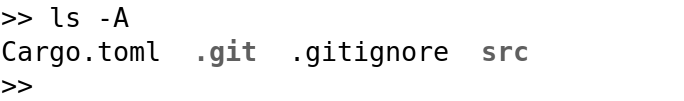
\includegraphics[width=0.5\textwidth]{img/figura_holacargo_bw.png}}
      \caption{Ficheros y carpetas creados en el directorio del proyecto \textit{hola\_cargo}, tras su creación por \textit{Cargo}}
      \label{fig_holacargo}
   \end{center}
\end{figure}

En la Figura \ref{fig_holacargo} se puede ver que se ha creado el fichero \texttt{Cargo.toml} \footnote{TOML es el acrónimo de <<\textit{Tom's Obvious, Minimal Language}>>. Este lenguaje está pensado para los ficheros de configuración. Su creador fue \textit{Tom Preston-Werner}.}. Este fichero contiene la información necesaria para compilar el programa. También se incluirían ahí las dependencias, si las hubiera. El contenido de dicho fichero, en el proyecto recién creado es similar al siguiente:
\begin{Codigo}
[package]
name = "hola_cargo"
version = "0.1.0"
edition = "2021"

# See more keys and their definitions at
# https://doc.rust-lang.org/cargo/reference/manifest.html

[dependencies]
\end{Codigo}

Las secciones de este fichero comienzan con un nombre de sección entre corchetes. La primera sección, \texttt{[package]}, contiene el nombre y la versión del programa y la edición de Rust utilizada para su creación. A continuación hay unos comentarios, que son las líneas que comienzan con el carácter \#. Finalmente, hay una sección \texttt{[dependencies]} inicialmente vacía.

Además del fichero \texttt{Cargo.toml}, en la carpeta del proyecto recién creado aparece un fichero \texttt{.gitignore} y una carpeta \texttt{.git}. Al crear un nuevo programa, \textit{Cargo} inicializa un repositorio \textit{GIT} para el mismo. Se pueden utilizar también otros gestores de versiones.

También se puede crear un nuevo proyecto Rust en un directorio donde ya exista un repositorio \textit{GIT}, mediante la orden \texttt{cargo init}. Puede teclear en la consola la orden \texttt{cargo new --help} para obtener más información o consultar el <<Libro de Cargo>> \citep{CargoBook} en la
documentación de Rust.

En el directorio del proyecto hay un directorio llamado \texttt{src} y, dentro de él, un fichero llamado \texttt{main.rs}. Si edita el fichero \texttt{main.rs} verá que contiene un código como el siguiente:
\begin{Codigo}
fn main() {
   println!("Hello, world!");
}
\end{Codigo}

Es la función \texttt{main()} con la misma instrucción \texttt{println!()} que se utilizó en el apartado anterior. Cada vez que \textit{Cargo} crea un nuevo programa, lo crea como un programa <<\textit{Hola Mundo}>> listo para funcionar.

Para compilar y ejecutar el programa hay que teclear en el terminal la siguiente instrucción:

{\centering\texttt{cargo run}\par}

Si vuelve a listar el directorio del proyecto verá que se ha creado una nueva carpeta llamada \texttt{target}. Dentro de ella hay otras carpetas y ficheros. El ejecutable creado está en la carpeta \texttt{target/debug} y lo podrá ejecutar en \textit{Linux} y \textit{macOS} con la instrucción siguiente:

{\centering\texttt{./target/debug/hola\_cargo}\par}

En \textit{Windows}, la instrucción que hay que teclear para ejecutar el programa es:

{\centering\texttt{.\textbackslash target\textbackslash debug\textbackslash hola\_cargo.exe}\par}

En el directorio del proyecto verá que también se ha creado un fichero \texttt{Cargo.lock}. Se trata de un fichero que utiliza el programa \textit{Cargo} para gestionar las versiones utilizadas de las dependencias. Dicho fichero lo mantiene de manera automática el programa \textit{Cargo} y el usuario no necesita modificarlo. Si tiene curiosidad, puede listar el fichero para ver su contenido.

Se puede compilar o construir el programa sin ejecutarlo, mediante la siguiente instrucción:

{\centering\texttt{cargo build}\par}

El comando \texttt{cargo build} admite diferentes opciones de compilación en combinación con las especificaciones del fichero \texttt{Cargo.toml}. Tienen que ver con la versión a construir, la realización de test y otras. Se recomienda consultar el ``\textit{Libro de Cargo}'' \citep{CargoBook} para ampliar la información al respecto.

A veces, la primera vez que se construye el programa o tras varias sesiones de trabajo consecutivas, puede suceder que el comando \texttt{cargo build} no funcione de la manera esperada. Una posible solución es ejecutar el comando \texttt{cargo clean}, que eliminará el directorio \texttt{target}. Tras esta limpieza, el comando \texttt{cargo build} debería volver a funcionar de manera adecuada.

Otra opción interesante es \texttt{cargo check}, que comprueba el código sin llegar a compilar el ejecutable. En programas extensos puede ser más rápido que compilar el programa completo.

En Rust, los programas se denominan ``\textit{crates}''. Hay dos tipos de \textit{crates}: programas binarios (ejecutables) y librerías. Los programas que hemos visto hasta ahora entran en la categoría de programas ejecutables. Para crear una librería, la orden que hay que teclear en el terminal es la siguiente:

{\centering\texttt{cargo new {-}{-}lib mi\_libreria}\par}

El programa \textit{Cargo} creará la estructura de directorios correspondiente. Dentro del directorio \textit{src} crea un fichero \textit{lib.rs} con el código inicial de la librería creada, que consiste en un test. 

\section{Código de los ejemplos}
\label{sec_codigo_ejemplos}
\noindent A lo largo de este texto se dan numerosos ejemplos de código. Sería muy farragoso crear un nuevo proyecto para cada ejemplo. Una manera más eficiente de probar el código de los ejemplos puede ser utilizar \textit{Cargo} para crear un proyecto genérico de nombre arbitrario y luego limitarse a cambiar el código de la función \textit{main()} por el código que aparece para cada ejemplo concreto. Tras ello, se puede comprobar el resultado ejecutando la orden \textit{cargo run}.

Otra forma de probar los ejemplos es el portal \textit{Rust Playground}, que permite probar los programas en línea y ofrece algunas opciones adicionales interesantes:

{\centering \texttt{https://play.rust-lang.org/} \par}

En algunos ejemplos, se incluye código que da lugar a errores de compilación, que se indicarán en los comentarios del código. Se hace a propósito, con fines didácticos y para que el lector pueda observar los mensajes de error que muestra el compilador de \textit{Rust}. Una de las características destacadas de \textit{Rust} es la calidad de los mensajes de error y las sugerencias para resolver dichos errores que ofrece el compilador. La lectura detenida de estos mensajes constituye también una valiosa fuente de aprendizaje.

A lo largo de los ejemplos se utilizan profusamente la instrucción \texttt{println!()} y la instrucción  \texttt{assert\_eq!()}. Se trata de macros del lenguaje. Las macros son un tipo especial de funciones; se diferencian de las funciones ordinarias en que el último carácter del nombre es el símbolo de exclamación ``\texttt{!}''. El uso básico de estas dos macros en los ejemplos se hace necesario. Se supone que el lector comprenderá rápidamente su funcionamiento cuando ejecute por sí mismo los ejemplos que se proponen. Se da a continuación una pequeña explicación de su funcionamiento:

\begin{itemize}
   \item \textbf{\texttt{println!()}:} esta macro permite hacer salidas por pantalla.
   Recibe una cadena de caracteres. Dentro de la cadena se pueden incluir \textit{especificaciones de formato}, que son una pareja de llaves `` \texttt{\{\}}``. En la salida, la pareja de llaves se sustituye por el valor de las variables que aparecen listadas tras la cadena de caracteres. Por ejemplo:
   
   \begin{Codigo}
      println!("La variable x vale {}", x);
   \end{Codigo}
   
   \vspace{0.8em}
   Esta instrucción escribirá en pantalla la cadena \texttt{"La variable x vale "}, seguida del valor que tenga en ese momento la variable \texttt{x}.
   
   \item \textbf{\texttt{assert\_eq!()}:} esta macro compara los valores de los resultados de las dos expresiones que recibe como parámetros. Si son iguales, no hace nada, pero si no lo son, interrumpe la ejecución del programa con un mensaje de error.
\end{itemize}

\section{Conceptos comunes en programación}
\noindent En la década de los años treinta del siglo XX, Alan Turing estableció los principios que debía cumplir un sistema de programación para poder resolver cualquier problema de computación. Traducido a los conceptos que se manejan en los lenguajes de programación actuales, se pueden resumir en tres condiciones:
\begin{itemize}
   \item \textbf{Asignación de variables:} las variables son nombres simbólicos (etiquetas) asociados a valores en memoria. Mediante el procedimiento de asignación, se asocia el nombre simbólico a un valor guardado en la memoria. De esta forma, una vez que se declara y se asigna valor a una variable, queda
   guardado en memoria y dicho valor se podrá utilizar en otra parte del programa, recuperándolo mediante el nombre de la variable
   
   \item \textbf{Bifurcaciones:} procedimiento que permite variar el flujo del programa, en base a condiciones lógicas
   
   \item \textbf{Bucles:} procedimiento que permite repetir cierto número de veces un bloque de código
\end{itemize}

Además de estos conceptos, casi todos los lenguajes permiten utilizar determinados tipos básicos de datos, permiten utilizar líneas de comentarios en el código fuente del programa y proporcionan la posibilidad de definir funciones.

En \textit{Rust} es importante distinguir entre las instrucciones que dan lugar a un valor y las que no. Se denominan \textit{declaraciones}, (\textit{statements}), las instrucciones que realizan alguna acción pero sin devolver ningún valor. Por ejemplo, la siguiente instrucción es una declaración.

\begin{Codigo}
   let x=7;
\end{Codigo}

Se denominan \textit{expresiones}, (\textit{expressions}), las instrucciones que dan lugar a un resultado. Por ejemplo, la siguiente instrucción es una expresión:

\begin{Codigo}
   x+y
\end{Codigo}

El concepto existe en todos los lenguajes, pero en algunos no es muy importante. En cambio, en \textit{Rust} es una diferencia que adquiere importancia en numerosas situaciones, como se irá viendo a lo largo de esta documentación.

Todos los conceptos de programación comentados en los párrafos precedentes son comunes a casi todos los lenguajes de programación, si bien cada uno los resuelve con diferente sintaxis o mediante procedimientos
específicos.

Otra particularidad común a todos los lenguajes es la existencia de palabras reservadas del lenguaje, que no se pueden utilizar como nombres de variables o funciones. Una vez más, cada lenguaje tiene su propio conjunto de palabras reservadas.

\section{Comentarios en los programas}
\label{sec_comentarios}
\noindent El código de los programas puede incluir comentarios informativos. Se puede hacer de dos maneras: comentarios de una línea o comentarios de bloque de varias líneas.

Los comentarios de línea, se añaden anteponiendo dos barras inclinadas \texttt{//} al texto que se quiera usar como comentario. Si las barras están al principio de la línea, toda la línea será un comentario. Si están tras alguna instrucción, el comentario será desde donde aparecen las barras inclinadas hasta el final de la línea.

También se pueden hacer comentarios de bloque, que abarquen varias líneas. Se hacen poniendo el bloque comentario entre los símbolos \texttt{/*} y \texttt{*/}. Todo lo que quede entre los dos símbolos, se tratará como un comentario:

\begin{Codigo}
   // Comentario de una línea
   let x = 2; // Comentario de parte de una línea
   /* Este es un comentario de bloque,
   que abarca varias líneas de texto.
   El criterio de estilo es poner los símbolos
   de apertura al principio de la primera línea,
   y los símbolos de cierre, al principio de la
   siguiente línea a la última de texto comentado
   */
\end{Codigo}

En general, el criterio de estilo al codificar programas en \textit{Rust} es utilizar comentarios con doble barra inclinada, incluso si ocupan más de una línea. En los ejemplos que acompañan a las explicaciones de los capítulos, se verá en numerosas ocasiones la utilización de comentarios.

A veces, los comentarios se utilizan para inutilizar algunas líneas de código y que no se ejecuten. Es una técnica habitual durante la depuración de los programas.

Hay otro tipo de comentarios que sirven para generar la documentación de los programas, pero que no se tratan en este curso. El lector interesado puede consultar la forma de documentar programas en el siguiente enlace:


{\centering\small \texttt{https://doc.rust-lang.org/rustdoc/how-to-write-documentation.html} \par}


% ---------------------------------------------------
% ---------------------------------------------------
\chapter{Elementos fundamentales del lenguaje Rust}
\label{ch_elementos_rust}
% ---------------------------------------------------
% ---------------------------------------------------
\IndiceCapitulo
\begin{Resumen}
La sintaxis del lenguaje Rust es similar a la de C o Java, con algunas diferencias que se irán indicando a lo largo del documento.

\smallskip

Rust dispone de una amplia colección de tipos de datos. En este texto se hará una introducción los siguientes:

\begin{enumerate}
   \item \textit{Tipos primitivos:} números enteros, números en coma flotante, valores booleanos, caracteres y el tipo unidad.
   \item \textit{Tipos compuestos:} arrays, vectores y tuplas.
   \item  \textit{Cadenas de caracteres}.
   \item \textit{Tipos personalizados:} estructuras y enumeraciones.
\end{enumerate}

Los tipos de datos básicos son similares a los de cualquier otro lenguaje, aunque Rust ofrece tipos enteros de 16 bytes, que no están disponibles en todos los lenguajes y, para los caracteres, se utilizan valores unicode. También es característico el tipo unitario, utilizado en expresiones que no devuelven ningún valor.

\smallskip

Los tipos compuestos, arrays y tuplas, en principio son similares a las que se pueden encontrar en otros lenguajes, si bien su conexión con los iteradores les confieren mayores posibilidades. Existen diferentes tipos para colecciones. Se tratarán los vectores, por ser los más sencillos y más habituales.

\smallskip

Hay varios tipos de datos para operar con cadenas de caracteres. Se utilizan valores unicode, lo que permite trabajar en cualquier idioma, incluso a nivel de nombres de identificadores. 

\smallskip

Las diferencias con otros lenguajes de programación son más evidentes en los tipos de datos personalizados: las estructuras y las enumeraciones. En Rust se trata de tipos de datos muy potentes que permiten incorporar funciones asociadas y, en el caso de las enumeraciones, unos patrones de coincidencia que posibilitan la utilización de técnicas de programación funcional.

\smallskip

También se tratarán en este capítulo conceptos como la asignación de variables, la declaración de mutabilidad, las construcciones habituales para bifurcaciones, bucles, la sintaxis básica para definir funciones y los traits.
 
\end{Resumen}


\section{Tipos de datos primitivos}

\subsection{Tipos para números enteros}
\label{sec_numeros_enteros}
\noindent Rust admite números enteros de 8, 16, 32, 64 y 128 bits, con signo o sin signo. Los tipos con signo se declaran poniendo una letra ``i'' y el número de bits; los números sin signo se declaran poniendo la letra ``u'' y el número de bits. 

Además, existen otros dos tipos denominados \textit{isize} y \textit{usize} que, según la plataforma para la que se esté desarrollando, tendrán un tamaño u otro. Se corresponden con el tamaño de los punteros en la plataforma. Por ejemplo, en plataformas con procesador de 32 bits, tienen 4 bytes de tamaño y, en plataformas de 64 bits, tienen un tamaño de 8 bytes. 

Cuando se escribe un número entero literal, sin especificar ninguna longitud de bits, se interpreta que es un número del tipo \textit{i32}. Los \textit{i32} son números enteros que ocupan 4 bytes en memoria. Su valor está entre -2147483648 y 2147483647 (entre menos dos mil millones y más dos mil millones, aprox). Es el tipo de número entero usado habitualmente por lenguajes como Java, por ejemplo. 

El siguiente ejemplo declara un número entero \textit{i32} y lo escribe en pantalla. A continuación, escribe el valor del mínimo número \textit{i32} y de máximo número \textit{i32}:

\vspace{0.7em}
\begin{Codigo}
let n = 127;
println!("El valor de n es {}", n);
println!("Mínimo:{} Máximo:{}", i32::MIN, i32::MAX);
\end{Codigo}

Observe la primera línea de código dentro de la función \textit{main()}:

{\centering \texttt{let n = 127;} \par}

Esta línea de código crea una variable de nombre \textit{n} y le asigna el valor 127. La cláusula \textit{let} se utiliza para declarar una variable. En este caso, se crea la variable \textit{n} y, en la misma línea de código, se le asigna el valor \textit{127}. El signo $=$ es el \textit{operador de asignación}: asigna el resultado de la expresión que aparece a la derecha del operador a la variable cuyo nombre aparece a la izquierda del operador. Más adelante se hablará más sobre creación y asignación de variables. La línea de código termina con \textit{punto y coma}.

En la línea de código que se ha analizado en el párrafo anterior, como no se ha especificado ningún tipo de datos y el valor literal es un entero, Rust interpreta que la variable \textit{n} es del tipo \textit{i32}, entero de 4 bytes.

Las siguientes líneas de código utilizan la macro \textit{println!()}. El funcionamiento de esta macro es similar al de la instrucción \textit{printf()} de los lenguajes Java o C: en la cadena entrecomillada se ponen especificaciones de formato que se sustituirán en la salida por el valor de las variables que aparecen a continuación de la cadena de caracteres. En este caso, la línea de código es:

{\centering \texttt{println!(``El valor de n es \{\}'', n);} \par}

La cadena de caracteres tiene un texto y una pareja de llaves. La pareja de llaves es la forma de especificar en Rust el formato de salida. En esa posición se incrustará el valor de la variable que aparece a continuación de la cadena de caracteres, la variable \textit{n}. Más adelante se verán formas de alterar el formato de salida. Si solo se ponen las dos llaves, el formato de salida será el que tiene definido Rust por defecto. Una vez más, la línea de código se termina con punto y coma.
\vspace{1em}

La siguiente línea de código es:

{\centering \texttt{println!("Mínimo:\{\} Máximo:\{\}", i32::MIN, i32::MAX);} \par}

En este caso, la cadena de caracteres de la macro \textit{println!()} tiene dos especificaciones de formato, dos parejas de llaves. Ahí se incrustará el valor de las variables que aparecen a continuación, que son \textit{i32::MIN} e \textit{i32::MAX}. Estas variables corresponden a los valores mínimo y máximo de los números del tipo \textit{i32}. Son constantes predefinidas en la librería de Rust. 

Observe cómo se accede a ellas: se pone el nombre del tipo de datos, dos veces dos puntos y el nombre de la constante. En Rust, \textit{dos veces dos puntos} es la forma de acceder a los valores estáticos de las librerías o de los tipos de datos definidos por el usuario. Java, por ejemplo, utiliza un solo punto para acceder a los valores. En Java, para acceder al valor mínimo del tipo \textit{int}, se habría escrito así:

{\centering \texttt{Integer.MIN\_VALUE} \par}

En Java, la constante se llama \textit{MIN\_VALUE} y es un atributo estático de la clase \textit{Integer}. En Java, para acceder a los métodos o atributos estáticos de una clase se utiliza el nombre de la clase, un punto y el nombre del atributo. En Rust, para acceder a los métodos o atributos estáticos se utilizan dos veces dos puntos. Se verá más adelante que, para acceder a los métodos o atributos \textit{de instancia}, se utiliza un solo punto, como en Java.

Cuando se quiere utilizar una variable de un tipo entero que no sea el \textit{i32}, hay que declarar explícitamente el tipo de datos. Para declarar que una variable es de un tipo de datos concreto se pueden utilizar dos procedimientos:

\begin{itemize}
   \item Declarando el tipo de datos a continuación del nombre de la variable, separado por dos puntos. Por ejemplo, la siguiente línea de código declara y asigna valor a una variable de nombre \textit{x} y del tipo \textit{u8}, o sea un entero sin signo de un byte de tamaño:
   
   {\centering \texttt{let x:u8 = 255;} \par}
   
   \item También se puede especificar el tipo de datos escribiendo el nombre del tipo  a continuación del valor literal, sin espacios. La siguiente línea de código sería equivalente a la anterior:
   
   {\centering \texttt{let x = 255u8;} \par}   
\end{itemize}

\subsection{Números en coma flotante}
\noindent Rust ofrece dos tipos de datos primitivos para números en coma flotante: \textit{f64} y \textit{f32}. Los valores del tipo \textit{f64} utilizan 8 bytes de almacenamiento en memoria; es el equivalente del tipo \textit{double} de otros lenguajes. Los valores del tipo \textit{f32} utilizan 4 bytes para el almacenamiento; es el tipo equivalente al \textit{float} de otros lenguajes. Como se sabe, los números \textit{f64} ofrecen una precisión aproximada de 15 decimales y los números \textit{f32} ofrecen una precisión aproximada de 8 decimales.

Las siguientes serían declaraciones y asignaciones válidas de variables de los tipos \textit{f64} y \textit{f32}:

\vspace{0.7em}
\begin{Codigo}
let a = 3.141592;
let b = 2.1e-3;
let c = 3.14f32;
let d: f32 = 3.1e5;
println!("{} {} {} {}", a, b, c, d);
\end{Codigo}
\vspace{1em}

El separador de decimales que se utiliza en los literales es el punto. Si se asigna a una variable un valor literal que incluya el punto decimal y no se específica otra cosa, Rust interpreta que la variable es del tipo \textit{f64}. Se puede utilizar la notación exponencial para escribir números literales.

Rust ofrece varias constantes predefinidas para números \textit{f64} o \textit{f32}. El siguiente código muestra algunos ejemplos:

\vspace{0.7em}
\begin{Codigo}
let a = std::f64::consts::PI;
let b = std::f32::consts::E;
let c = std::f64::consts::SQRT_2;
println!("{:.12} {:.6} {:.2}", a, b, c);
\end{Codigo}

Observe que se ha utilizado la especificación de formato ``\{:.n\}'' para fijar el número de decimales que se muestran en la salida. 

Hay dos juegos independientes de constantes para valores \textit{f64} y \textit{f32}. Se pueden consultar en los siguientes enlaces:

{\centering \texttt{https://doc.rust-lang.org/std/f64/consts/index.html} \par}   

{\centering \texttt{https://doc.rust-lang.org/std/f32/consts/index.html} \par}   

\subsection{Valores booleanos}
\noindent El tipo de datos se denomina \textit{bool}. Las variables del tipo bool pueden tomar el valor \textit{true} o \textit{false}. No se pueden utilizar el número 1 o el número 0 para sustituir a las palabras \textit{true} o \textit{false}.

El siguiente código podría servir para declarar una variable del tipo \textit{bool}:

{\centering \texttt{let si = true;} \par}   

\section{El tipo unidad}
\noindent El \textit{tipo unidad} o \textit{tupla vacía} se representa por ``()'' y sirve para indicar que una expresión devuelve un valor vacío. En Rust, es importante la distinción entre \textit{expresiones} y \textit{declaraciones}. Las declaraciones son instrucciones o líneas de código que no devuelven ningún valor, mientras que las expresiones son instrucciones o líneas de código que devuelven algún valor. Como se irá comprobando a lo largo del curso, Rust utiliza preferentemente expresiones que devuelven valores, aunque puede suceder que el valor devuelto sea el valor unidad o valor vacío ``()''.

\subsection{Caracteres}
\noindent El tipo utilizado para almacenar caracteres individuales es el tipo \textit{char}. Cada carácter es un valor \textit{Unicode}, por lo que es posible guardar no solo caracteres, sino todo tipo de símbolos. Una consecuencia es que un carácter puede ocupar más de un byte. El siguiente ejemplo muestra cómo usar valores \textit{unicode}:

\vspace{0.7em}
\begin{Codigo}
let a = 'a';
let epsilon = '\u{0190}';
let esqui = '\u{26f7}';
let emoticono = '\u{1f601}';
println!("{} {} {} {}", a, epsilon, esqui, emoticono);
\end{Codigo} 

\section{Tipos de datos compuestos}

\subsection{Arrays}
\noindent En programación, un \textit{array} es un tipo de datos que agrupa en una misma entidad una colección de valores del mismo tipo de datos que se guardan en memoria en posiciones consecutivas; se puede acceder a cada valor individual utilizando un índice. A cada valor de un array se le suele denominar \textit{elemento} o \textit{componente} del array.

En Rust, los arrays tienen que tener un tamaño y un tipo de datos conocidos en tiempo de compilación. Una vez creado un array, se puede acceder a los elementos con la notación de índices entre corchetes, siendo el primer elemento el de índice 0. El siguiente código declara algunos arrays e imprime algunos elementos individuales:

\vspace{0.7em}
\begin{Codigo}
let a = [1, 2, 3, 4, 5];
println!("{}", a[2]); // Imprime 3
let b: [f32;3]; // Declara un array de 3 elementos del tipo f32
let c: [u8;3] = [0, 101, 255]; // Crea array de 3 u8
println!("{:?}", c); // Imprime [0, 101, 255]
\end{Codigo}

Observe, en la última línea de código, la especificación de formato ``\{:?\}''. Algunos tipos de datos, como es el caso de los arrays, se pueden imprimir utilizando dicha especificación de formato\footnote{La especificación de formato ``\{:?\} se puede utilizar con los tipos de datos que implementan el \textit{trait Debug}. A este formato se le suele denominar \textit{pretty-print}.}. 

\subsection{Tuplas}
\noindent Las tuplas son un tipo de datos que une en una sola entidad varios elementos que no tienen por qué ser del mismo tipo de datos. Se declaran con paréntesis (no corchetes como los arrays). Al igual que sucede con los arrays, hay que definir en tiempo de compilación el tamaño y el tipo de datos de cada una de las componentes de la tupla. Una vez creada una tupla, no se puede cambiar su tamaño ni el tipo de datos de sus componentes. Los elementos individuales pueden ser accedidos con la notación \textit{variable-punto-índice}, como se hace en el siguiente código:

\vspace{0.7em}
\begin{Codigo}
let a: (u8, u8, u8) = (255, 127, 255);
println!("{}", a.1); // Imprime 127
\end{Codigo}

\subsection{Vectores}
\noindent Los vectores son similares a los arrays pero, a diferencia de estos, pueden cambiar de tamaño de manera dinámica (en tiempo de ejecución). Todos los elementos de un vector tienen que ser del mismo tipo de datos. Para poder modificar las componentes o para añadir o eliminar componentes de un vector, será necesario declararlo \textit{mutable}. Más adelante se explicará cómo hacerlo. Se puede acceder a los elementos individuales con notación de índice entre corchetes. 

El siguiente ejemplo crea un vector de 3 componentes del tipo \textit{f64} utilizando la macro \textit{vec![]}, lo imprime en pantalla y luego imprime uno de sus elementos:

\vspace{0.7em}
\begin{Codigo}
let v = vec![3.14, 6.28, 3.14];
println!("{:?}", v); // Imprime [3.14, 6.28, 3.14]
println!("{}", v[1]);
\end{Codigo}

El tipo de datos es \textit{Vec<T>}. Se trata de un tipo de datos parametrizado en el que \textit{T} representa el tipo de datos de las componentes del vector. En Rust, es habitual denominar a \textit{T} un \textit{tipo genérico}. El tipo \textit{Vec<T>} ofrece numerosos métodos utilitarios que se pueden consultar en la documentación de la librería estándar, en la siguiente dirección:

{\centering \texttt{https://doc.rust-lang.org/std/vec/struct.Vec.html} \par}   

\section{Tipos de datos personalizados}
\label{sec_tipos_personalizados}

\subsection{Estructuras}
\noindent Las estructuras definen un tipo de datos que incorpora en la misma variable varias componentes de distintos tipos. Se puede acceder al valor individual de un campo de una estructura mediante la notación \textit{variable-punto-nombre\_campo}

El siguiente ejemplo crea una estructura \textit{Point}, con dos campos \textit{x} e \textit{y} del tipo \textit{i32}. En el programa principal se crea una instancia de dicha estructura y se imprime en pantalla el valor de sus campos:

\vspace{0.7em}
\begin{Codigo}
struct Point {
   x: i32,
   y: i32
}
fn main() {
   let origen = Point{x: 0, y: 0};
   println!("{} {}", p.x, p.y); // Imprime 0 0
}
\end{Codigo}

Observe la sintaxis para crear la instancia \textit{p} de la estructura, poniendo entre llaves los nombre de campos y los valores que se asignan a los mismos.

Se pueden definir funciones asociadas al tipo de datos, lo que convierte a las estructuras de Rust en un tipo de datos similar a las clases de otros lenguajes. Más adelante, cuando se expliquen las funciones, se explicará cómo crear funciones asociadas a las estructuras.

Las estructuras descritas contienen campos con nombre, pero también es posible crear estructuras con campos sin nombre, que se suelen denominar \textit{estructuras tuplas}, como se hace en el siguiente ejemplo:

\vspace{0.7em}
\begin{Codigo}
struct Color(i32, i32, i32);
struct Point(i32, i32, i32);

fn main() {
   let black = Color(0, 0, 0);
   let origin = Point(0, 0, 0);
}
\end{Codigo}

En este caso, las instancias de \textit{Point} y de \textit{Color} son distintos tipos de datos, aunque los dos consten de tres números \textit{i32}. No se puede utilizar una variable de un tipo en sustitución de una variable del otro tipo. Para acceder a los campos, se utiliza el nombre de variable, un punto y el índice que ocupa, como en las tuplas:

{\centering \texttt{let x = origin.0;} \par}

Otra variante es la denominada \textit{estructuras unidad}, que no tienen campos. Pueden ser útiles para depuración de código o en otros contextos en los que solo se necesita \textit{marcar} la existencia de un tipo sin datos:

\vspace{0.7em}
\begin{Codigo}
struct SinCampos;

fn main() {
   let x = SinCampos;
}
\end{Codigo}

\subsection{Enumeraciones}
\noindent En programación, las enumeraciones son un tipo de datos que agrupa en una misma entidad un conjunto de valores con nombre. A cada uno de los valores que componen la enumeración se le denomina \textit{variante} o \textit{miembro} de la enumeración. Las variables de dichos tipos pueden tomar solo uno entre los valores de las variantes definidas. En un programa, se asocian variables a dichas variantes, permitiendo la comparación entre ellas.
 
En algunos lenguajes, las enumeraciones son simplemente una forma de dar nombre a algunas constantes, asociando cada variante con un número entero, por ejemplo. Esto permite hacer comparaciones entre distintas variables. El siguiente código muestra un ejemplo de utilización en C:

\vspace{0.7em}
\begin{Codigo}
enum Level {
   LOW,
   MEDIUM,
   HIGH
};
int main() {
   enum Level nivel = MEDIUM;
   if (nivel == LOW) {
      // haz_una_cosa()
   } else {
      // haz_otra_cosa()
   }  
}
\end{Codigo}

Combinando este tipo de enumeraciones con las estructuras, sería posible distinguir unas instancias de otras. Otros lenguajes, como Java, añaden algunas capacidades extra a las enumeraciones, convirtiéndolas en un tipo especial de clase de objetos con propiedades y métodos asociados. 

En Rust, las enumeraciones son un tipo de datos muy potente que permite asociar un valor de cualquier tipo de datos a cada una de las variantes de la enumeración o asociar funciones al tipo de datos, de manera similar a lo que se hace con las estructuras. 

Rust utiliza dos enumeraciones especiales, \textit{Result} y \textit{Option}, para gestionar los errores de ejecución o los valores devueltos por las funciones. Estas dos características, en combinación con la instrucción \textit{match}, proporcionan a Rust algunos patrones de diseño característicos de la programación funcional, como se irá viendo. 

La sintaxis de la declaración de una enumeración en Rust es similar a la de C o Java. El siguiente ejemplo declara el tipo \textit{Color} y crea un valor de dicho tipo:

\vspace{0.7em}
\begin{Codigo}
enum Color {
   Rojo,
   Verde,
   Azul
}
fn main() {
   let color = Color::Verde;
}
\end{Codigo}

Al tipo, en este caso \textit{Color}, se le denomina \textit{identificador} o simplemente \textit{tipo}. A cada uno de los posibles valores que pueden tomar las variables, \textit{Rojo}, \textit{Verde} o \textit{Azul}, se les denomina \textit{variantes} o \textit{miembros} del tipo \textit{Color}, como ya se ha indicado.

Para poder realizar comparaciones entre variables del tipo creado, se debe indicar al compilador que implemente para dicho tipo el \textit{trait PartialEq}, lo que equivale a imponer que se pueden utilizar los operadores \texttt{==} y \texttt{!=}. Esto se consigue escribiendo una anotación \texttt{\#derive[PartialEq]} en el tipo de datos creado. Con esto, sería posible hacer una comparación entre dos variables del tipo \textit{Color}, como se hace en el siguiente código:

\vspace{0.7em}
\begin{Codigo}
#[derive(PartialEq)]
enum Color {
   Rojo,
   Verde,
   Azul
}

fn main() {
   let color_1 = Color::Rojo;
   let color_2 = Color::Azul;  
   if color_1 == color_2 {
      // haz_algo()
   }
}
\end{Codigo} 

Al compilar el código anterior, se muestra un mensaje de advertencia indicando que la variante \textit{Color::Verde} no se utiliza nunca en el código. 

Cada variante de una enumeración puede llevar asociado un valor de cualquier tipo de datos, que además puede ser diferente para cada variante.

El siguiente ejemplo utiliza una enumeración para definir un color. La variante \textit{RGB} define un color mediante sus proporciones de \textit{Red}, \textit{Green} y \textit{Blue}; la variante \textit{RGBA} añade una componente con el nivel de transparencia \textit{Alpha} y la variante \textit{CMYK}  combina \textit{Cyan}, \textit{Magenta}, \textit{Yellow} y \textit{Key} (\textit{Negro}). 

\vspace{0.7em}
\begin{Codigo}
#[derive(PartialEq)]
enum Color {
   RGB(u8, u8, u8),
   RGBA(u8, u8, u8, u8),
   CMYK { cyan: u8, magenta: u8, yellow: u8, key: u8 },
}
\end{Codigo}

En el código anterior, se utilizan dos maneras diferentes de asociar valores a las variantes del tipo \textit{Color}. En las variantes \textit{RGB} y \textit{RGBA}, se ha asociado una tupla de enteros tipo \textit{u8}, en un caso con tres valores y en el otro con cuatro. En cambio, la variante \textit{CMYK} utiliza una estructura de campos con nombre. En un caso real, lo lógico sería utilizar un mismo criterio con todas las variantes del tipo.

Definido el tipo \textit{Color}, se podrían crear variables y hacer comparaciones:

\vspace{0.7em}
\begin{Codigo}
#[derive(PartialEq)]
enum Color {
   RGB(u8, u8, u8),
   RGBA(u8, u8, u8, u8),
   CMYK { cyan: u8, magenta: u8, yellow: u8, key: u8 },
}

fn main() {
   let alice_blue = Color::RGB(240, 248, 255);
   let naranja = Color::RGBA(243, 156, 18, 255);
   println!("{}", alice_blue==naranja); // false
}
\end{Codigo}

\vfill\null

También es posible utilizar los valores asociados a cada variante, utilizando instrucciones \textit{match}\footnote{La instrucción \textit{match} se explicará en el Apartado \ref{sec_bifurcaciones}. El lector necesitará comprender dicho apartado para comprender el ejemplo que se muestra.}:

\vspace{0.7em}
\begin{Codigo}
match alice_blue {
   Color::RGB(red, green, blue) => {
      println!("Red:{red} Grren:{green} Blue:{blue}");
   },
   _ => println!("No es RGB")
}
\end{Codigo}

Se pueden definir funciones asociadas al tipo de datos. El siguiente ejemplo implementa una función que imprime los valores asociados a cada color:

\vspace{0.7em}
\begin{Codigo}
impl Color {
   pub fn to_hex(&self) -> String {
      match self {
         Color::RGB(red, green, blue) => {
            format!("#{:X}{:X}{:X}", red, green, blue)
         },
         _ => format!("No implementado"),
      }
   }
}
\end{Codigo}

\section{Cadenas de caracteres}
\noindent Las cadenas de caracteres tienen un tratamiento especial en todos los lenguajes de programación y, en general, un tratamiento diferente en cada lenguaje. Como se ha indicado, en Rust los caracteres individuales son valores Unicode y las cadenas de caracteres también están formadas por valores Unicode. Se usan dos tipos de datos para cadenas de caracteres:

\begin{itemize}
   \item \textbf{\&str:} se usa para los \textit{literales entrecomillados}. Cuando se asigna a una variable un literal entrecomillado, el tipo asignado es \textit{\&str}, que no está afectado por las reglas de propiedad que se verán más adelante, aunque sí que está afectado por las reglas de \textit{vida útil} que afectan a las referencias. 
   \item \textbf{String:} es el tipo de datos que se utiliza para las cadenas de caracteres propiamente dichas. Es un tipo afectado por las reglas de propiedad.
\end{itemize}

Las variables del tipo \textit{\&str} se crean asignando un valor entre comillas dobles:

{\centering \texttt{let nombre = ``Ramón Requena'';} \par}

Las variables del tipo \textit{String} disponen de método para su creación a partir de un literal entrecomillado:

{\centering \texttt{let nombre = String::from(``Ramón Requena'');} \par}

En Rust, el tipo \textit{String} es muy potente y con una gran cantidad de métodos utilitarios. Se puede consultar su documentación en el siguiente enlace:

{\centering \small \url{https://doc.rust-lang.org/std/string/struct.String.html} \par}

\section{Criterios para los nombres de los identificadores}
\noindent Los nombres válidos de los identificadores deben seguir la norma \textit{Unicode Standard Annex \#31} \citep{UAX31Unicode}. Se admiten caracteres Unicode, por lo que es posible utilizar la letra \textit{ñ} u otros caracteres de otros idiomas. También está permitido usar el guion bajo, el símbolo de dólar u otros. No obstante, para facilitar la internacionalización del código, se recomienda utilizar solo los caracteres del alfabeto inglés, en mayúsculas o minúsculas, números y el guion bajo. 

Además, se siguen las siguientes reglas:

\begin{itemize}
   \item El lenguaje distingue entre mayúsculas y minúsculas, por lo que la variable \textit{X} mayúscula es diferente de la variable \textit{x} minúscula.
   \item Los números pueden formar parte del nombre de un identificador, pero no pueden ser el primer carácter del mismo.
   \item El guion bajo sí que puede ser el primer carácter del identificador, pero es costumbre que los nombre que comienzan con guion bajo se utilicen para identificadores que no se van a utilizar posteriormente.
\end{itemize}

En Rust, es costumbre utilizar para los identificadores de variables, nombres de funciones y otros el criterio llamado \textit{snake case}, que consiste en utilizar palabras en minúsculas separadas por guiones bajos. Ejemplos de la utilización de este criterio podrían ser los siguientes:

{\centering \texttt x \hspace{2em} min\_value \hspace{2em} get\_sum()\par}

Cuando se trata de constantes, se utiliza el llamado \textit{screaming snake case}, en el que las palabras se escriben con letras en mayúsculas, por ejemplo:

{\centering \texttt VALOR\_RESIDUAL \hspace{2em} SCREAMING\_SNAKE\_CASE \par}

Los nombres de los tipos de datos, como los nombres de estructuras o enumeraciones, en cambio, utilizan el criterio \textit{camel case}, con las palabras en mayúsculas y sin espacios ni guiones bajos entre ellas, por ejemplo:

{\centering \texttt Color \hspace{2em} LineaDePuntos \par}

Aunque se podría utilizar cualquier otro criterio en los nombres de los identificadores, la utilización de este código de conducta facilita la lectura del código por distintos programadores.

Si necesita más información al respecto, puede consultar la referencia del lenguaje en la siguiente dirección:

{\centering \small \url{https://doc.rust-lang.org/reference/identifiers.html} \par}

\section{Mutabilidad}
\noindent En Rust, las variables son \textit{inmutables} por defecto: una vez que se ha asignado un valor, no es posible modificarlo. El código siguiente no compila, la variable \textit{x} es inmutable y no es posible asignarle un nuevo valor:

\vspace{0.7em}
\begin{Codigo}
fn main() {
   let x = 8.5;
   x = 3.4; // ¡ERROR, no compila, x es inmutable!
}
\end{Codigo}


Para que una variable sea \textit{mutable}, hay que indicarlo explícitamente en la declaración de la variable utilizando la cláusula \textit{mut}, como se hace en el siguiente código:

\vspace{0.7em}
\begin{Codigo}
fn main() {
   let mut v = vec![1, 2, 3];
   v[1] = 100;
   v.push(200);
}
\end{Codigo}

\vspace{1em}

Una cosa diferente es redefinir una variable ya existente utilizando \textit{let}, lo que se denomina \textit{shadowing}. En realidad, lo que se hace es crear una nueva variable con el mismo nombre. La variable anterior queda inaccesible. La nueva variable no tiene por qué ser del mismo tipo que la original:

\vspace{0.7em}
\begin{Codigo}
fn main() {
   let x: f64 = 3.14;
   println!("{}", x); // Imprime 3.14
   let x: u8 = 255;
   println!("{}", x); // Imprime 255
}
\end{Codigo}

\section{Obtener el tipo de una variable}
\noindent La librería estándar de Rust ofrece una función que permite obtener el nombre del tipo de datos de una variable. Se muestra su uso con un ejemplo:

\vspace{0.7em}
\begin{Codigo}
let v = vec![1, 2, 3, 4, 5];
println!("{}", std::any::type_name_of_val(&v)); 
// Imprime alloc::vec::Vec<i32>
\end{Codigo}

\section{El operador de asignación}
\noindent Hay un operador fundamental en cualquier lenguaje que ya se ha utilizado anteriormente, dando por hecho que el lector tiene una comprensión, al menos intuitiva, de su funcionamiento: el \textit{operador de asignación}. 

En Rust, el operador de asignación utiliza el símbolo $=$ (igual). A la derecha del símbolo igual se escribe una expresión, esto es, código que devuelve un resultado; a la izquierda del operador se pone el nombre de una variable. Lo que hace el operador es asignar a la variable cuyo nombre aparece a la izquierda del signo igual el resultado de la expresión que aparece a la derecha del mismo. La línea de código de una asignación tiene que terminar en punto y coma. 

El ejemplo más sencillo de expresión es un literal, por ejemplo un número. El operador asignará el valor de dicho número a la variable cuyo nombre figura a la izquierda del operador. Observe el siguiente ejemplo:

{\centering \texttt{v = 5;} \par}

A la izquierda del signo igual figura el nombre de la variable \textit{v} y, a la derecha, el número 5. Como resultado del operador, el valor 5 se asignará a la variable \textit{v}. 



Para poder utilizar una línea de código como la anterior, es necesario que la variable \textit{v} haya sido declarada con anterioridad, con una instrucción \textit{let} o con una instrucción \textit{let mut}. En el primer caso, la asignación solo puede hacerse una vez; en el segundo caso, la asignación se puede hacer más de una vez. Es habitual hacer la declaración de la variable y la asignación de valor en la misma línea de código:

{\centering \texttt{let v = 5;} \par}

Un detalle imprescindible en toda asignación es que el resultado de la expresión que aparece a la derecha del operador tiene que ser del mismo tipo de datos que la variable a la que se le asigna. En este caso, el tipo de datos es \textit{i32} y queda establecido en el valor del literal; en  otros casos, será necesario establecer el tipo de datos, bien en la declaración de la variable o bien en el propio literal, como se explicó en el Apartado \ref{sec_numeros_enteros}.

Las expresiones que aparecen a la derecha del operador de asignación son cualquier código que devuelva un resultado. En la mayoría de los lenguajes de programación, las expresiones están formadas por una combinación de literales, operadores e identificadores de otras variables o funciones. En Rust, hay construcciones del lenguaje que también son expresiones y devuelven un resultado, como los bloques de instrucciones del tipo \textit{if} o los bloques correspondientes a los bucles (\textit{loop}, \textit{for} y \textit{while}). Más adelante se verán ejemplos de estos usos del operador de asignación.

Otro caso de asignación que hay que tener en cuenta es cuando la expresión que aparece a la derecha del operador de asignación es el nombre de otra variable. En ese caso, según el tipo de datos de las variables, hay dos comportamientos posibles. Como se verá en el Apartado \ref{sec_propiedad}, hay tipos de datos que funcionan con semántica \textit{Copy} y otros tipos de datos que funcionan con semántica \textit{Move}. 

En las asignaciones (y también en el paso de parámetros a funciones), los tipos que funcionan con \textit{Copy} realizan una copia del valor de una variable en la otra, quedando dos variables útiles, con valores iguales. Esto sucede con los tipos primitivos, los arrays y las tuplas cuyos elementos son tipos primitivos y cualquier otro tipo de datos que implemente el \textit{trait Copy}. El siguiente sería un ejemplo utilizando números \textit{f64}:

\vspace{0.7em}
\begin{Codigo}
let x: f64 = 0.75;
let y = x;
assert_eq!(x, 0.75);
assert_eq!(y, 0.75);
\end{Codigo}

Tras la asignación, las dos variables \textit{x} e \textit{y} siguen existiendo.

En cambio, si las variables son de un tipo que funciona con \textit{Move}, tras la asignación la variable original deja de ser accesible y la propiedad del valor pasa a la nueva variable:

\vspace{0.7em}
\begin{Codigo}
let v = vec![1, 2, 3];
let w = v;
assert_eq!(w, vec![1, 2, 3]);
assert_eq!(v, vec![1, 2, 3]); // ERROR, v ya no es accesible
\end{Codigo}

\section{Otros operadores}
\noindent Además del operador de asignación, hay otros operadores que también son habituales en cualquier lenguaje de programación:

\begin{itemize}
   \item Operadores aritméticos.
   \item Operadores relacionales o de comparación.
   \item Operadores lógicos.
   \item Operadores de asignación compuestos.
\end{itemize}

En todos los casos, estos operadores representan una forma abreviada de utilizar ciertas funciones que reciben uno o dos argumentos y devuelven un resultado calculado en base al valor de dichos argumentos. Los argumentos se suelen llamar también \textit{operandos}.

En Rust, el tipo de datos de los operandos tiene que ser el mismo. No se pueden operar valores de diferentes tipos de datos. El resultado puede ser del mismo tipo que los operandos o no, según el operador que se esté utilizando.

\subsection{Operadores aritméticos}
\noindent Los operadores aritméticos utilizan dos argumentos de tipo numérico y devuelven como resultado un valor numérico del mismo tipo de datos. Se resumen en la Tabla \ref{tabla_operadores_aritmeticos}.

\begin{center}
   \begin{mytable}[label=tabla_operadores_aritmeticos]{\centering\footnotesize Operadores aritméticos}
      \footnotesize
      \begin{tabular}{c l}
         \hline
         \textbf{Operador} & \textbf{Significado} \\ \hline
         $+$ & Suma \\
         $-$ & Resta \\
         $*$ & Producto \\
         $/$ & División \\
         $\%$ & Resto de la división \\
      \end{tabular}
   \end{mytable}
\end{center}


Como se ha dicho, los dos operandos tienen que ser del mismo tipo de datos y el resultado también lo será. No es posible, or ejemplo, sumar un entero \textit{i32} con un entero \textit{u8}:

\vspace{0.7em}
\begin{Codigo}
let x : i32 = 12;
let y : u8 = 5;
println!("{}", x+y); // ERROR, no son del mismo tipo
\end{Codigo}

Rust ofrece la cláusula \textit{as} para hacer \textit{casting} de unos tipos de datos a otros:

\vspace{0.7em}
\begin{Codigo}
let x : i32 = 12;
let y : u8 = 5;
println!("{}", x as u8 + y); // Imprime 17
println!("{}", x + y as i32); // Imprime 17
\end{Codigo}

En una expresión en la que se combinen varios operadores, el interprete del lenguaje opera de izquierda a derecha, pero hay elementos que alteran el orden de las operaciones. Por ejemplo, las expresiones que estén encerradas entre paréntesis, las llamadas a funciones o los nombre de otras variables, se ejecutan antes y su resultado se sustituye en la expresión. También se ejecutan antes los productos, las divisiones y el resto que las sumas y restas. 

Se muestran a continuación algunos ejemplos:
\begin{align*}
& 5 + 3 + 4 \quad \rightarrow \quad 8 + 4 \quad \rightarrow \quad 12\\
& 5 + 3 * 4 -1 \quad \rightarrow \quad 5 + 12 - 1 \quad \rightarrow \quad 17 - 1 \quad \rightarrow \quad 16\\
& (5 + 3) * 4 -1 \quad \rightarrow \quad 8 * 4 - 1 \quad \rightarrow \quad 32 - 1 \quad \rightarrow \quad 31\\
& 3 + 5 {\:} \% {\:}  2 \quad \rightarrow \quad 3 + 1 \quad \rightarrow \quad 4\\
\end{align*}

\subsection{Operadores relacionales o de comparación}
\noindent Los operadores \textit{relacionales}, también llamados \textit{de comparación}, reciben dos operandos de tipo numérico y devuelven un valor \textit{bool:} \textit{true} o \textit{false}. Se resumen en la Tabla \ref{tabla_operadores_relacionales}.

\begin{center}
   \begin{mytable}[label=tabla_operadores_relacionales]{\centering\footnotesize Operadores relacionales o de comparación}
      \footnotesize
      \begin{tabular}{c l}
         \hline
         \textbf{Operador} & \textbf{Significado} \\ \hline
         $<$ & Menor que \\
         $<=$ & Menor o igual que \\
         $>$ & Mayor que \\
         $>=$ & Mayor o igual que \\
         $==$ & Igual (\textit{Igual-Igual}) \\
         $!=$ & No igual \\
      \end{tabular}
   \end{mytable}
\end{center}

Como se puede ver en la Tabla \ref{tabla_operadores_relacionales}, algunos operadores constan de dos caracteres. Merece mención especial el operador $==$ (\textit{igual-igual)}), que no hay que confundir con el operador de asignación $=$ (\textit{igual}). Esta confusión, frecuente entre estudiantes que están iniciándose en programación, da lugar a algunos \textit{bugs}\footnote{En programación, hay distintos tipos de errores. Por una parte, están los errores de sintaxis o de codificación que hacen que el programa no compile. Suelen ser los errores más fáciles de depurar. También hay errores de ejecución que, según el tipo concreto, pueden ser más o menos difíciles de depurar. Por último están los \textit{bugs}, errores en la lógica del programa; en los \textit{bugs}, el programa compila y se ejecuta sin interrupciones, pero los resultados no coinciden con lo que cabría esperar. Suelen ser los más difíciles de depurar.} difíciles de depurar.

En cuanto al operador \texttt{!=} (\textit{no igual}), hay otros lenguajes que utilizan otra sintaxis, por ejemplo, en MATLAB se utiliza $\sim =$.

Cuando en una expresión se combinan varios operadores, se operan de izquierda a derecha. Si aparecen operadores aritméticos y operadores de comparación, los operadores aritméticos se ejecutan antes que los de comparación. A continuación se muestran algunos ejemplos:
\begin{align*}
   & 5 > 2 + 3 \quad \rightarrow \quad 5 > 5 \quad \rightarrow \quad false\\
   & 5 + 1 > 2 + 3 \quad \rightarrow \quad 6 > 2 + 3 \quad \rightarrow \quad 6 > 5 \quad \rightarrow \quad true\\
\end{align*}


\subsection{Operadores lógicos}
\noindent Los operadores \textit{lógicos} reciben uno o dos operandos del tipo \textit{bool} y devuelven un resultado del tipo \textit{bool}. Se resumen en la Tabla \ref{tabla_operadores_logicos}.

\begin{center}
   \begin{mytable}[label=tabla_operadores_logicos]{\centering\footnotesize Operadores lógicos}
      \footnotesize
      \begin{tabular}{c l}
         \hline
         \textbf{Operador} & \textbf{Significado} \\ \hline
         $\&\&$ & AND : \textit{true}, si los dos operandos son \textit{true}, \textit{false} en caso contrario \\
         $||$ & OR : \textit{true}, si al menos uno de los operadores es \textit{true}, \textit{false} en caso contrario \\
         $!$ & NOT : \textit{true}, si el operando es \textit{false}, \textit{false} en caso contrario\\
      \end{tabular}
   \end{mytable}
\end{center}

En Rust, los operadores lógicos aplican el llamado \textit{short-cicuiting}, esto es, evalúan el primer operando y si queda resuelto el resultado, no evalúan el segundo. Por ejemplo, en un \textit{AND}, si el primer operando es \textit{false}, el resultado es \textit{false} cualquiera que sea el valor del segundo operando. En el operador \textit{OR}, si el primer operando es \textit{true}, el resultado es \textit{true} con seguridad.

En cierto sentido, el operador lógico \textit{AND} se podría equiparar al operador aritmético producto y el operador lógico \textit{OR} se podría equiparar a la suma. De hecho, si en una expresión aparecen operadores \textit{AND} y operadores \textit{OR}, se ejecutan primero los \textit{AND}. El operador \textit{NOT} tiene precedencia sobre los otros operadores lógicos: primero se ejecuta los operadores \textit{NOT}, luego los operadores \textit{AND} y, por último, los operadores \textit{OR}.
 
Cuando en una expresión aparecen operadores lógicos y operadores de comparación, los operadores de comparación se operan antes que los lógicos (recuerde que los operadores aritméticos se ejecutan antes que los de comparación). 

Un caso paradigmático de esta regla de precedencia de los operadores de comparación sobre los lógicos es la condición para indicar que un número está dentro de determinado intervalo. En notación algebraica, un ejemplo podría ser:
\[x \in (a, b) \Rightarrow a < x < b\]
La expresión algebraica $a<x<b$ encierra dos comparaciones y un operador \textit{AND}: \textit{a es menor que x Y x es menor que b}. En Rust, se podría poner:

{\centering \texttt{a<x \&\& x<b} \par}

El orden de precedencia de los operadores hace innecesarios los paréntesis, aunque también se podrían utilizar para facilitar la lectura.

\subsection{Operadores compuestos de asignación}
\noindent Son operadores que realizan una operación aritmética y una asignación. Se resumen en la Tabla \ref{tabla_operadores_compuestos_asignacion}.

\begin{center}
   \begin{mytable}[label=tabla_operadores_compuestos_asignacion]{\centering\footnotesize Operadores compuestos de asignación}
      \footnotesize
      \begin{tabular}{c l}
         \hline
         \textbf{Operador} & \textbf{Significado} \\ \hline
         $+=$ & Suma y asignación \\
         $-=$ & Resta y asignación \\
         $*=$ & Producto y asignación\\
         $/=$ & División y asignación\\
         $\%=$ & Resto y asignación\\
      \end{tabular}
   \end{mytable}
\end{center}

\section{Funciones de los tipos en coma flotante}
\noindent Todos los tipos de datos que se han visto en los apartados anteriores disponen de funciones utilitarias que se pueden consultar en la documentación de la librería estándar:

{\centering \texttt{https://doc.rust-lang.org/std/index.html} \par}

En este apartado se van a comentar las funciones asociadas a los tipos \textit{f64} y \textit{f32}, por ser de uso frecuente en cálculos matemáticos. La totalidad de los métodos se pueden consultar en los siguientes enlaces:

{\centering \texttt{https://doc.rust-lang.org/std/primitive.f64.html} \par}

{\centering \texttt{https://doc.rust-lang.org/std/primitive.f32.html} \par}

Lo primero que hay que indicar es que hay un juego de funciones para operar con valores \textit{f32} y otro juego de funciones para operar con valores \textit{f64}. Como se comentó en el caso de los operadores, no se pueden mezclar tipos, cuando se opera con valores \textit{f64} hay que utilizar funciones del tipo \textit{f64} y análogamente cuando se opera con valores \textit{f32}.

Lo siguiente que suele sorprender al trabajar con funciones matemáticas en Rust es la forma de invocarlas. No se llama a una función y se le pasa el argumento entre paréntesis, se invoca con la notación \textit{valor-punto-función}, de la misma forma que se llama a las funciones asociadas a otros tipos de datos. Por ejemplo, para calcular la raíz cuadrada de \textit{4.0} se haría de la siguiente forma:

{\centering \texttt{4.0f64.sqrt()} \par}

Observe que ha sido necesario especificar el tipo de datos concreto, \textit{f64}, en el literal del valor \textit{4.0}. Si no se hace, el compilador indica que hay ambigüedad entre la función \textit{sqrt()} para \textit{f64} y la función \textit{sqrt()} para \textit{f32}. Si el valor ya tuviera el tipo de datos asignado, no sería necesario hacerlo así:

{\hspace{7em} \texttt{let x: f64 = 4.0;} \par}

{\vspace{-0.7em}\hspace{7em} \texttt{let y = x.sqrt();} \par}

Normalmente, uno está acostumbrado a trabajar con lenguajes en los que las funciones reciben los parámetros entre los paréntesis. Por ejemplo, en Java se habría escrito algo así:

{\hspace{7em} \texttt{double x = 4.0;} \par}

{\vspace{-0.7em}\hspace{7em} \texttt{double y = Math.sqrt(x);} \par}

En un primer momento, la forma de escribir las funciones en Rust se hace un poco rara. Pero es una cuestión de cambiar la forma en la que se interpretan las expresiones anteriores. En el caso de la función \textit{sqrt(x)}, la leeríamos como \textit{``raíz cuadrada de x''}. En el caso de la sintaxis de Rust, \textit{x.sqrt()}, es mejor leerlo como ``\textit{al valor x se le aplica la función raíz cuadrada}''. 

Puede parecer artificioso, pero piense en el caso de varias funciones compuestas, por ejemplo una expresión del tipo:

\[\sqrt{\sin{(x^2)}}\]

En realidad, la forma de operar una expresión de ese tipo es de dentro hacia afuera: se calcula el cuadrado de \textit{x}, luego el seno de ese resultado y, finalmente, la raíz cuadrada del resultado. Se leería: ``\textit{raíz cuadrada del seno de x al cuadrado}''. En Java se escribiría:

\vspace{0.3em}
{\centering \texttt{Math.sqrt(Math.sin(x*x))} \par}
\vspace{0.3em}

En el caso de Rust, esa expresión se escribiría así:

\vspace{0.3em}
{\centering \texttt{(x*x).sin().sqrt()} \par}
\vspace{0.3em}

Se podría leer como: ``\textit{Se calcula x al cuadrado, se le aplica la función seno y, al resultado, se le aplica la función raíz cuadrada}''. En la sintaxis se recoge el orden en el que se realizan las operaciones, la forma en la que se componen las funciones que se van aplicando. Es una forma más \textit{declarativa} de escribir las operaciones, aunque se aleje de la forma en la que estamos acostumbrados a escribir esas expresiones.

De hecho, una vez que uno se acostumbra a escribir las operaciones de esta manera, se convierte en natural y lógica y, lo que se hace extraño y artificioso, es la forma clásica de escritura de esas mismas expresiones. En realidad, las dos formas de escribir las expresiones se corresponden con las dos formas de expresar la composición de funciones en matemáticas:

\[f(g(h(x)))  \quad \rightarrow \quad (h \cdot g \cdot f) (x) \]

Por último, hacer notar cómo se encadenan varias operaciones en Rust con la notación punto. A lo largo de este escrito se verán otras ocasiones en las que se utiliza esta composición de operaciones, una tras otra, simplemente poniendo el punto.

No obstante, si el lector no consigue acostumbrarse a esta forma de escribir las funciones y prefiere a toda costa utilizar la forma tradicional de invocar funciones, siempre podría codificar las que necesite para poder invocarlas de la manera tradicional, como se hace en el siguiente programa:

\vspace{0.7em}
\begin{Codigo}
fn main() {
   let x: f64 = 0.75;
   let y = sqrt(sin(x));
   println!("{y:.4}"); // Imprime 0.8256
}
fn sin(x: f64) -> f64 {
   x.sin()
}
fn sqrt(x: f64) -> f64 {
   x.sqrt()
}
\end{Codigo}


\section{Bifurcaciones}
\label{sec_bifurcaciones}

\subsection{Bifurcaciones \textit{if...else}}
\noindent La sintaxis es similar a la de otros lenguajes. La condición tiene que ser una expresión que devuelva un valor \textit{bool}, no se admiten números ni otros tipos de datos. Como detalle, no es necesario poner la condición entre paréntesis. El siguiente código muestra un ejemplo de \textit{if} con cláusula \textit{else}:

\vspace{0.7em}
\begin{Codigo}
fn main() {
   let n = 3;
   if n < 5 {
      println!("Condición verdadera");
   } else {
      println!("Condición falsa");
   }
}
\end{Codigo}

Es posible utilizar bifurcaciones \textit{if} sin rama \textit{else} y también con ramas múltiples del tipo \textit{else if}, como se hace en el siguiente ejemplo:

\vspace{0.7em}
\begin{Codigo}
fn main() {
   let n = 3;
   if n==0 {
      println!("Cero");
   } else if n%2==0 {
      println!("Par");
   } else {
      println!("Impar");
   }
}
\end{Codigo}

Si bien la sintaxis es similar a la de otros lenguajes, hay una diferencia fundamental en cuanto al comportamiento de la instrucción. En Rust, la instrucción \textit{if} es una expresión, no una declaración. Esto quiere decir que cada rama de un \textit{if}, devuelve un valor. El valor que devuelven las ramas de los ejemplos anteriores es el valor unidad, (). 

Al tratarse de una expresión, es posible usar un \textit{if} en la parte derecha de una asignación, como se hace en el siguiente ejemplo:

\vspace{0.7em}
\begin{Codigo}
let n = 3;
let is_par = if n%2==0 {true} else {false};
\end{Codigo}

Observe que los bloques \textit{if} no necesitan punto y coma al final del bloque pero, en el ejemplo anterior, sí que es necesario, por tratarse de una  asignación.

Las dos ramas del \textit{if} tienen que devolver el mismo tipo de datos, si no se produce un error de compilación. El siguiente código daría error:

\vspace{0.7em}
\begin{Codigo}
let n = 3;
let is_par = if n%2==0 {n} else {"impar"};
\end{Codigo}

\subsection{Bifurcaciones \textit{match}}
\label{sec_match}
\noindent La otra construcción que permite gestionar bifurcaciones es el bloque \textit{match}, similar al \textit{case} o al \textit{switch} de otros lenguajes. En un bloque \textit{match}, se evalúa un valor entre varias opciones. Se denominan \textit{ramas}, a cada una de las líneas de bifurcación en función de los posibles valores. Los bloques \textit{match} son bifurcaciones \textit{en paralelo}, en las que el código sale por una rama de entre varias\footnote{En realidad no son exactamente bifurcaciones en paralelo, pues las condiciones se evauan una tras otra hasta que se encuentra una en la que hay coincidencia.}.

El compilador obliga a que la instrucción \textit{match} compruebe todos los posibles valores de la variable que se está evaluando. En el siguiente ejemplo se muestra la sintaxis de la instrucción:

\begin{Codigo}
fn main() {
   let x = 10;
   let resto = x%2;
   match resto {
      0 => println!("Par"),
      _ => println!("Impar"),
   }
}
\end{Codigo}

El símbolo del guion bajo \textit{\_} que se utiliza en las ramas de \textit{match} se interpreta como <<\textit{cualquier valor}>>. Es habitual escribir el símbolo \textit{\_}, pero se podría utilizar cualquier otro nombre de variable, como \textit{other} o cualquier otro. El motivo de utilizar el guion bajo es que el compilador de \textit{Rust} genera un aviso cuando se declara una variable y no se utiliza, pero este aviso no se genera si el nombre de la variable es el guion bajo \textit{\_} o comienza por un guion bajo \textit{\_}.

La construcción \textit{match} no solo funciona con enteros, se pueden probar valores de cualquier tipo. En el caso de los números en coma flotante, la necesidad de comprobar todos los valores posibles puede hacer necesario establecer condiciones lógicas del tipo <<\textit{menor que}>> u otras similares. Para ello, se pone la condición con un \textit{if} después de la declaración de la variable en la rama correspondiente, como se hace en el siguiente ejemplo:

\begin{Codigo}
fn main() {
   let x = 2.5;
   match x {
      valor if valor<10.0 => println!("{valor} < 10.0"),
      valor if valor==10.0 => println!("{valor} == 10.0"),
      _ => println!("{x} > 10.0"),
   };
}
\end{Codigo}

También se puede utilizar la coincidencia de patrones con tipos personalizados, por ejemplo con una tupla:

\begin{Codigo}
match (1, "Hello") {
   (i, _) if i < 0 => println!("Negative integer: {}", i),
   (_, s) => println!("{} World", s),
}
\end{Codigo}

Un uso muy habitual de los bloques \textit{match} es para comprobar las opciones posibles cuando el resultado es una enumeración del tipo \textit{enum}, como se verá más adelante.
 
\section{Bucles}
\label{sec_bucles}
\noindent Rust tiene tres tipos de bucles: \textit{loop}, \textit{while} y \textit{for}.

El bucle \textit{loop} se ejecuta de manera indefinida, salvo que se le indique explícitamente que termine:

\vspace{0.7em}
\begin{Codigo}
fn main() {
   loop {
      println!("Bucle infinito!");
   }
}
\end{Codigo}

Si ejecuta el código anterior, tendrá que pulsar \textit{CTRL + C} para terminar.

Las cláusulas \textit{break} y \textit{continue} se pueden utilizar dentro de cualquier bucle para alterar el flujo normal del mismo. La cláusula \textit{continue} ignora las restantes instrucciones de la iteración e inicia una nueva iteración. La cláusula \textit{break} ignora el resto del código en el bucle y el resto de las iteraciones que pudiera haber pendientes y salta a la siguiente instrucción de código tras el bucle.

Los bucles \textit{while} también tienen una sintaxis similar a la de otros lenguajes, con la salvedad, si acaso, de que no es necesario encerrar la condición entre paréntesis.

\vspace{0.7em}
\begin{Codigo}
fn main() {
   let mut contador = 0;
   while contador < 5 {
      println!("{contador}");
      contador += 1;
   }
}
\end{Codigo}


Los bucles \textit{for} se utilizan para recorrer colecciones:

\vspace{0.7em}
\begin{Codigo}
fn main() {
   let a = [10, 20, 30, 40, 50];
   for elemento in a {
      println!("El valor es: {elemento}");
   }
}
\end{Codigo}

Combinando los bucles \textit{for} con los \textit{Range} (\textit{rango}), es posible generar muchos tipos de bucles con una sintaxis más declarativa que la de sus equivalentes bucles \textit{while}. Por ejemplo, el bucle contador se podría codificar de la siguiente forma:

\vspace{0.7em}
\begin{Codigo}
fn main() {
   for contador in 0..4 {
      println!("{contador}");
   }
}
\end{Codigo}

El código resultante, no solo es más declarativo que su equivalente \textit{while}, además no es necesario hacer mutable la variable contador.

Los rangos implementan el \textit{trait Iterator} y otros, lo que les proporciona numerosos métodos de utilidad que pueden servir para definir distintos tipos de bucles. Por ejemplo, el siguiente ejemplo usa los números del rango en orden inverso y de dos en dos:

\vspace{0.7em}
\begin{Codigo}
fn main() {
   for contador in (0..8).rev().step_by(2) {
      println!("{contador}");
   }
}
\end{Codigo}

\vspace{1em}

En Rust, los bucles también son expresiones. Para que un bucle devuelva un valor, se utiliza la cláusula \textit{break}. El valor devuelto será el resultado de la expresión que aparezca a continuación del \textit{break}. 

\vspace{0.7em}
\begin{Codigo}
   fn main() {
      let mut contador = 0;
      let result = loop {
         contador += 1;
         if contador == 10 {
            break contador * 2;
         }
      };
      println!("{result}"); // Imprime 20
   }
\end{Codigo}

La línea de código donde aparece \textit{break} se puede acabar con punto y coma o sin él, pero observe el punto y coma que cierra la asignación a \textit{result}. Ahí sí es necesario el punto y coma, pues se trata de una asignación.


\section{Funciones}
\label{sec_funciones}
\noindent De manera similar a la de otros lenguajes, las funciones se definen mediante una línea de signatura seguida del cuerpo de la función entre llaves. La signatura utiliza la cláusula \textit{fn} seguida de un nombre válido de función, la lista de parámetros entre paréntesis y, si devuelven algún valor, se pone una \textit{flecha} ``->'' seguida del tipo de datos del valor devuelto. A continuación, entre llaves, irá el cuerpo de la función.

\vspace{0.7em}
\begin{Codigo}
fn nombre(param_1: tipo_1, ...) -> tipo_devuelto {
   // Instrucciones del cuerpo de la función
}
\end{Codigo}

Para devolver un valor dentro del cuerpo de la función, no es necesario utilizar la cláusula \textit{return}, aunque puede usarse; es suficiente dejar una expresión sin terminar en punto y coma; el resultado de dicha expresión se utilizará como valor devuelto. Solo se puede devolver un valor, aunque puede ser de cualquier tipo, incluyendo arrays, estructuras u otros.

Un ejemplo podría ser el siguiente:

\vspace{0.7em}
\begin{Codigo}
fn por_dos(x: i32) -> i32 {
   2*x
}
\end{Codigo}

En el ejemplo anterior, la función se llama \textit{por\_dos}, recibe un parámetro de nombre \textit{x} del tipo \textit{i32} y devuelve un valor del tipo \textit{i32}. El cuerpo de la función es una sola línea de código que multiplica por 2 el valor de \textit{x} que recibe. Esa línea de código se finaliza sin punto y coma, por lo que el resultado de la expresión \textit{2*x} será el valor devuelto por la función.

\subsection{Funciones asociadas a las estructuras y enumeraciones}
\noindent Cuando se implementan funciones asociadas a una estructura o una enumeración, se hace dentro de un bloque \textit{impl}. Hay dos tipos de funciones asociadas a las estructuras y enumeraciones:

\begin{itemize}
   \item \textit{Estáticas:} asociadas al tipo de datos, no a las instancias de dicho tipo. Se invocan usando el nombre del tipo, dos veces dos puntos y el nombre de la función.
   \item \textit{De instancia:} el primer parámetro debe ser la palabra clave \textit{self}, que identifica a la instancia concreta que invoca al método. El parámetro \textit{self} se puede especificar de tres formas: \textit{self}, \textit{\&self} y \textit{\&mut self}, según se pase la propiedad, una referencia al valor o una referencia mutable al valor. 
\end{itemize}

El siguiente ejemplo, crea la estructura \textit{Point} e implementa dos métodos: uno estático llamado \textit{new()}, que hace las veces de constructor y otro de instancia, llamado \textit{sum()}, que devuelve la suma de las componentes del \textit{Point}. En el programa principal se crea una instancia de \textit{Point} y se invocan ambos métodos:

\vspace{0.7em}
\begin{Codigo}
struct Point {
   x: i32,
   y: i32
}

impl Point {
   fn new(x: i32, y: i32) -> Point {
      Point{x: x, y: y}
   }
   fn sum(&self) -> i32 {
      self.x + self.y
   }
}
fn main() {
   let p = Point::new(3, 2); // Crea una instancia de Point 
                             // y la asigna a la variable p
   let suma = p.sum();       // Suma las componentes de p
   println!("{}", suma);     // Imprime 5
}
\end{Codigo}

Observe que, en el método \textit{sum()}, se utiliza para el primer parámetro la forma \textit{\&self}, que es una referencia a la instancia que invoca el método, para no consumir la propiedad de la misma. Es la forma habitual de hacerlo y se comprenderá mejor cuando se explique el concepto de propiedad.

Observe también que, en el método \textit{new()}, el nombre de los parámetros coincide con el nombre de los campos de \textit{Point}. En estos casos se podría omitir el nombre del campo en la asignación de valores, haciendo:

\vspace{0.7em}
\begin{Codigo}
fn new(x: i32, y: i32) -> Point {
   Point{x, y}
}
\end{Codigo}

Observe, por último, la forma de invocar los dos métodos: el método estático con el nombre del tipo y dos veces dos puntos y el método de instancia con el nombre de variable y un solo punto.

En el caso de las enumeraciones, la forma de implementar métodos es igual que en el caso de las estructuras.

\subsection{Closures}
\noindent Son funciones, frecuentemente anónimas, declaradas \textit{inline} dentro del contexto de otra función y que pueden acceder a las variables de dicho contexto.

Las closures utilizan dos barras verticales, de la misma forma que las funciones ordinarias utilizan los paréntesis. Entre las barras verticales se ponen los nombres de los parámetros. En la mayoría de los casos, el compilador es capaz de inferir el tipo de los parámetros y no es necesario especificarlo. A continuación, se pone el código de la closure que, si solo consta de una línea, no es necesario encerrarlo entre llaves.

El siguiente ejemplo muestra una closure:

\vspace{0.7em}
\begin{Codigo}
let suma_uno = |x| x+1;
println!("{}", suma_uno(5)); // Imprime 6
\end{Codigo}

En el ejemplo, se declara una closure y se asigna a la variable \textit{suma\_uno}; se trata de una closure que recibe un argumento \textit{x} y devuelve \textit{x+1}.

Esta inferencia del tipo de datos de los parámetros en las closures puede permitir desarrollar closures para tipos genéricos. El siguiente código define una closure que recibe un parámetro \textit{x}. Al no especificar el tipo de datos de \textit{x}, la closure se puede utilizar con un valor entero o con una cadena de caracteres. Eso sí, el primer uso que se haga de la closure definirá el tipo de datos de \textit{x} y ya solo se podrá usar la closure con ese tipo de datos.

\vspace{0.7em}
\begin{Codigo}
fn main() {
   let f = |x| x;
   let s = f(String::from("hello"));
   let n = f(5); // ERROR, x ha quedado fijado a  tipo String 
}
\end{Codigo}

En el código anterior, el primer uso que se haga de la closure fijará el tipo de datos del parámetro para todos los usos subsiguientes. Si se hubiera usado primero con un valor entero, el uso posterior con una cadena de caracteres habría resultado en un error de compilación. 

Una característica de las closures es que pueden acceder a las variables del contexto en el que ha sido definida la closure. Según la forma en la que se realice dicho acceso, Rust establece tres tipos de closures:

\begin{itemize}
   \item Acceso por referencia: \textit{\&T}. Da lugar a closures del tipo \textit{Fn}.
   \item Acceso por referencia mutable: \textit{\&mut T}. Son closures del tipo \textit{FnMut}.
   \item Acceso por valor: \textit{T}. Según el tipo de datos de \textit{T}, la closure puede tomar la propiedad del mismo. En este caso la closure es del tipo \textit{FnOnce}.
\end{itemize}

En cada caso, Rust trata de asignar a la closure el tipo menos restrictivo que sea posible. Toda función es al menos \textit{FnOnce}. 

Hay que tener en cuenta que, para acceder a una variable del contexto, no es necesario especificar su nombre como parámetro de la closure. Los parámetros formales que se indican entre las barras verticales de la closure se refieren a argumentos que se recibirán en la invocación de la closure.

En el siguiente código, la closure utiliza una referencia a la variable \textit{x}. Es un ejemplo de closure del tipo \textit{Fn}:

\vspace{0.7em}
\begin{Codigo}
fn main() {
   let x = 10;
   let cuadrado = || {x*x};
   println!("{}", cuadrado(x)); // Imprime 100
}
\end{Codigo}

El siguiente ejemplo utiliza una referencia mutable a la variable \textit{x} del contexto. Se trata de una closure del tipo \textit{FnMut}. Es necesario declarar como mutables la variable \textit{x} y la closure \textit{incrementa\_x}:

\vspace{0.7em}
\begin{Codigo}
fn main() {
   let mut x = 10;
   let mut incrementa_x = || x+=1;
   incrementa_x();
   println!("{}", x); // Imprime 100
}
\end{Codigo}

La siguiente closure, en cambio, solo se puede ejecutar una vez, pues la variable \textit{v} se \textit{consume}, esto es, la propiedad se pasa a una variable local de la closure. Es un ejemplo de closure del tipo \textit{FnOnce}\footnote{El concepto de \textit{propiedad} de los valores se explicará en el Capítulo \ref{ch_propiedad}. Es posible que algunos de los conceptos que se están explicando en relación con las closures sea necesario releerlos tras leer dicho capítulo, a fin de comprenderlos mejor.}:

\vspace{0.7em}
\begin{Codigo}
fn main() {
   let v = vec![1, 2, 3];
   let consume_x =  || {let w = v;};
   consume_x();
   consume_x(); // ¡ERROR, v se ha movido fuera de su contexto!
}
\end{Codigo}

Se puede usar la cláusula \textit{move} para que la closure tome la propiedad del valor de una variable del contexto. Esto no impide que la closure se ejecute más de una vez, pero impide volver a utilizar dicha variable fuera de la closure:

\vspace{0.7em}
\begin{Codigo}
fn main() {
   let x = vec![1, 2, 3];
   let captura_x =  move || println!("{:?}", x);
   captura_x();
   captura_x();
   println!("{:?}", x); // ERROR, x se ha movido a la closure 
}
\end{Codigo}

Cuando se utiliza una variable del contexto dentro de una closure, se está compartiendo la propiedad de manera inmutable o de manera mutable. Dicha circunstancia estará activa mientras lo esté la closure y se regirá por las reglas generales sobre la forma de compartir referencias. Así, si se comparte una referencia mutable a un valor del contexto, no pueden existir simultáneamente otras referencias, ni mutables ni inmutables al mismo valor. 

Observe el siguiente ejemplo:

\vspace{0.7em}
\begin{Codigo}
fn main() {
   let mut x = vec![1, 2, 3];
   let mut modifica_x =  || {x.push(4); println!("{:?}", x)};
   
   modifica_x(); // Referencia mutable
   x.push(5);    // Referencia mutable
   println!("{:?}", x); // Referencia inmutable
}
\end{Codigo}

El código anterior sí que compila, a pesar de que se utilizan dos referencias mutables (\textit{modifica\_x()} y \textit{x\_push(5)}) y una referencia inmutable (\textit{printf!()}). Ninguna de las referencias compartidas se intenta utilizar por segunda vez después de haber usado otras. Así, si se hace una segunda llamada a \textit{modifica\_x()} después de haber utilizado la referencia inmutable o la otra referencia mutable, como se hace en el siguiente código, el compilador señalará dos errores: uso simultáneo de dos referencias mutables y uso simultáneo de una referencia inmutable mientras existe una referencia mutable:

\vspace{0.7em}
\begin{Codigo}
fn main() {
   let mut x = vec![1, 2, 3];
   let mut modifica_x =  || {x.push(4); println!("{:?}", x)};
   modifica_x();                                              
   x.push(5); // Segundo uso de una referencia mutable        
   println!("{:?}", x); // Uso de una referencia inmutable    
   modifica_x(); // Esta línea hace saltar los errores  
}
\end{Codigo}

Este segundo uso de \textit{modifica\_x()} hace ver al compilador que, entre los dos usos, la referencia mutable está activa y, por tanto, no permite la utilización entre medias de otras referencias, ni mutables ni inmutables.

Observe el siguiente código:

\vspace{0.7em}
\begin{Codigo}
fn main() {
   // Se declara y asigna x en el contexto
   let mut x = 10.9;
   // f accede al valor de x
   let f = || {return x};
   // Se modifica el valor de x en el contexto
   let x = 17.0;
   
   // f() sigue usando el antiguo valor de x
   println!("{:?}", f()); // Imprime 10.9
   // Dentro del contexto, x ha cambiado de valor
   println!("{v:?}");     // Imprime 17.0
}
\end{Codigo}

Cuando una closure accede a una variable del contexto, lo hace al valor que tenía dicha variable en el momento de declarar la closure. Si con posterioridad a la declaración de la closure se modifica el valor de la variable, la closure seguirá utilizando el valor que tenía la variable cuando se declaró la closure. El código del ejemplo anterior muestra claramente esta circunstancia.


El uso de closures es un patrón habitual en Rust. Son útiles en diversas situaciones:

\begin{itemize}
   \item Se pueden usar como argumentos de otras funciones.
   \vspace{0.5em}
   \item Se usan profusamente con los iteradores, en métodos como \textit{map()}, \textit{filter()} y otros.
   \vspace{0.5em}
   \item Se pueden usar como campos de una estructura y definir un comportamiento de la misma.
\end{itemize}

El uso de funciones como parámetros de otras funciones se verá más adelante. El código que sigue sería un ejemplo del tercer uso indicado. Se trata de una estructura que simboliza un \textit{botón} que llama a una closure cuando se pulsa:

\vspace{0.7em}
\begin{Codigo}
struct Button<F> {
   callback: F,
}

impl<F: Fn()> Button<F> {
   fn new(callback: F) -> Self {
      Self { callback }
   }
   fn click(&self) {
      (self.callback)();
   }
}

fn main() {
   let button = Button::new(|| println!("¡Botón pulsado!"));
   button.click();  // Imprime: ¡Botón pulsado!
}
\end{Codigo}

\section{Traits}
\label{sec_traits}
\noindent La palabra inglesa \textit{trait} se puede traducir por \textit{rasgo}, \textit{característica}, \textit{atributo} o \textit{cualidad}. Los \textit{traits} de \textit{Rust} son similares a los \textit{interfaces} existentes en otros lenguajes. Los \textit{traits} definen, de manera abstracta, las funcionalidades que deben implementar los tipos de datos adscritos al \textit{trait}. También sirven para limitar qué tipos concretos forman parte de un genérico. Para no dar lugar a errores de interpretación, a lo largo del
texto se utilizará la palabra \textit{trait} en inglés.

Las librerías del lenguaje \textit{Rust} incluyen muchos \textit{traits} predefinidos. Cada tipo de datos definido en el lenguaje implementa algunos de esos \textit{traits}. Por ejemplo, el \textit{trait} \textit{Iterator} define métodos como \textit{next()} o \textit{count()}. Los tipos de datos que implementan el \textit{trait} \textit{Iterator} implementan dichos métodos. En la librería estándar hay numerosos ejemplos de \textit{traits} definidos en el lenguaje.

Definir un \textit{trait} consiste en definir la signatura de una serie de métodos. La declaración y definición de un \textit{trait} se hace con la palabra clave \textit{trait}, seguida del nombre asignado a dicho \textit{trait}. A continuación, entre llaves, se lista la signatura de los métodos que deberán implementar los tipos que se adhieran a dicho \textit{trait}. La definición de un \textit{trait} se hace de la siguiente manera:

\begin{Codigo}
trait NombreDelTrait {
   ... signatura de los métodos del trait ...
}
\end{Codigo}

Por convenio, los \textit{traits} se nombran en mayúsculas siguiendo el criterio \textit{Camel Case}, con la primera letra de cada palabra en mayúsculas. Todos los tipos de datos que implementen el \textit{trait} deberán tener definido el código de dichos métodos.

Para definir la implementación de un \textit{trait} por parte de determinado tipo de datos, se utiliza la palabra clave \textit{impl} seguida del nombre del \textit{trait}, la palabra clave \textit{for} y el nombre del tipo de datos:

\begin{Codigo}
impl NombreDelTrait for NombreDelTipoDeDatos {
   ... métodos del trait ...
}
\end{Codigo}

Para ilustrar la forma de definir y utilizar los \textit{traits}, se va a desarrollar un ejemplo que simula un termostato capaz de accionar varios dispositivos:

\begin{Codigo}
trait Regulable {
   fn activar(&self);
   fn desactivar(&self);
}
struct Termostato;
impl Termostato {
   fn activa_disp<T: Regulable>(&self, dispositivo: &T) {
      dispositivo.activar();
   }
   fn desactiva_disp<T: Regulable>(&self, dispositivo: &T) {
      dispositivo.desactivar();
   }
}
\end{Codigo}

En primer lugar, se define el \textit{trait} \textit{Regulable} que tiene dos métodos llamados \textit{activar()} y \textit{desactivar()}. Cualquier dispositivo que tenga que ser accionado por el \textit{Termostato} deberá implementar dicho \textit{trait}. La estructura \textit{Termostato} tiene unos métodos para activar y desactivar los dispositivos, que son los que utiliza para manejar los aparatos. Estos métodos reciben como parámetro una referencia a un valor de un tipo genérico que implemente el \textit{trait} \textit{Regulable}. Esto garantiza que el dispositivo que reciban dichos métodos, implementará \textit{activar()} y \textit{desactivar()}, con lo que podrán ser manejados por el \textit{Termostato}.

En el código se puede ver cómo se especifica que un tipo genérico debe implementar determinado \textit{trait}: se ponen dos puntos tras la letra \textit{T} del genérico y, a continuación, el nombre del \textit{trait} que debe implementar; si tuviera que implementar  más de un \textit{trait}, se pone la lista de \textit{traits} separados por el símbolo $+$. Cuando se limitan los tipos genéricos permitidos para un parámetro a aquellos tipos que implementan determinados \textit{traits} se dice que se han impuesto \textit{trait bounds} a los parámetros.

A continuación se muestra el código de dos de dichos dispositivos: \textit{Radiador} y \textit{Ventilador}:


\begin{Codigo}
struct Radiador;

impl Regulable for Radiador {
   fn activar(&self) {
      println!("Radiador encendido");
   }
   fn desactivar(&self) {
      println!("Radiador apagado");
   }
}

struct Ventilador;

impl Regulable for Ventilador {
   fn activar(&self) {
      println!("Ventilador en marcha");
   }
   fn desactivar(&self) {
      println!("Ventilador parado");
   }
}
\end{Codigo}

Se puede observar cómo se ha implementado el código concreto de los métodos \textit{activar()} y \textit{desactivar()} para los tipos de datos \textit{Radiador} y \textit{Ventilador}: se define un bloque \textit{impl} que implementa los métodos \textit{activar()} y \textit{desactivar()} del \textit{trait}, con las instrucciones concretas para el tipo de datos correspondiente.

Por último, se muestra la función \textit{main()}, donde se crea un \textit{Termostato} que acciona un \textit{Radiador} y un \textit{Ventilador}:

\begin{Codigo}
fn main() {
   let tato = Termostato;
   let radiador = Radiador;
   tato.activar_dispositivo(&radiador);
   let ventilador = Ventilador;
   tato.activar_dispositivo(&ventilador);
   tato.desactivar_dispositivo(&radiador);
   tato.desactivar_dispositivo(&ventilador);
}
\end{Codigo}

Solo se puede implementar un \textit{trait} en un tipo si el \textit{trait} o el tipo son locales al código. Por ejemplo, se puede implementar el \textit{trait} \textit{Display} de la librería \textit{std} en un tipo perteneciente al programa que se esté desarrollando. También se podría implementar dentro de un programa el
\textit{trait} \textit{Regulable} para el tipo \textit{Vec<T>} de la librería \textit{std}. Lo que no se puede es implementar \textit{traits} externos en tipos externos. Por ejemplo, no se puede implementar el \textit{trait Display} en el tipo \textit{Vec<T>}, pues los dos son externos al código del programa que se esté desarrollando.

\subsection{Herencia en \textit{traits}}
\label{sec_herencia_traits}
\noindent \textit{Rust} no es un lenguaje orientado a objetos, aunque tiene elementos que permiten simular algunas de las características de la programación orientada a objetos. No existen objetos como tales, pero las estructuras pueden tener datos y métodos asociados, con lo que pueden suplir algunas de las funcionalidades que se asignan a los objetos en otros lenguajes. 

\textit{Rust} no dispone del mecanismo de herencia entre tipos de datos, pero sí que permite implementar la herencia en los \textit{traits}. Cuando se establece que un \textit{trait B} es derivado a partir de otro \textit{trait A}, los tipos de datos que implementen el \textit{trait B} derivado, están obligados a implementar los métodos que establece el \textit{trait A} del que deriva.

El siguiente ejemplo muestra el mecanismo de herencia de \textit{traits}. Se define el \textit{trait Mapa} que deriva del \textit{trait Dibujable}:

\begin{Codigo}
trait Dibujable {
   fn dibuja(&self);
}
trait Mapa : Dibujable {
   fn bounding_box(&self) -> (i32, i32, i32, i32);
}
\end{Codigo}

Los tipos que implementen el \textit{trait Mapa} deberán implementar el método \textit{dibuja()} del \textit{trait Mapa} y el método \textit{bounding\_box()} del \textit{trait Dibujable}.

\subsection{Diferencias entre \textit{traits} e \textit{interfaces}}
\noindent \textit{Rust} no es un lenguaje orientado a objetos. Sin embargo, observando los códigos anteriores, se puede ver que la utilización de estructuras y enumeraciones combinadas con \textit{traits} y genéricos permite realizar una programación similar a la programación orientada a objetos. No se dispone del mecanismo de herencia de tipos, pero sí que se dispone de un mecanismo de herencia de \textit{traits}, que permite un tipo de programación más flexible, como se comentó en el Apartado \ref{sec_adios_poo}.

Los traits de \textit{Rust} son similares a los \textit{interfaces} existentes en otros lenguajes, como en Java, por ejemplo. Hay algunas diferencias, no obstante, que conviene destacar:
\begin{itemize}
   \item En \textit{Rust} está definida la herencia entre \textit{traits}, pero no
   existe ningún mecanismo de herencia entre tipos de datos. Esto quiere decir que
   se puede definir un \textit{trait} \textit{B} que deriva de un \textit{trait}
   \textit{A}, y los tipos que quieran implementar el \textit{trait} \textit{B} deberán implementar también el \textit{trait} \textit{A}. Pero no hay ningún mecanismo de herencia entre los tipos asociados con la implementación de uno u otro \textit{trait}. 
   
   En programación orientada a objetos, esto implica que los tipos de datos
   utilizan la composición, no la herencia. Esto no es malo; de hecho, en programación orientada a objetos suele ser recomendable utilizar la composición frente a la herencia.
   
   \item Como ya se ha indicado, se pueden crear \textit{traits} para tipos externos al programa, aunque no se tenga acceso a los tipos.
   
   \item Los \textit{traits}, en sí mismos, no pueden ser el valor devuelto por un
   método, como sucede con los \textit{interfaces} en Java, por ejemplo. Para eso hay que devolver \textit{trait objects}.
\end{itemize}

\blankpage

% ------------------------------------------------------------
\chapter{Propiedad de los valores}
\label{ch_propiedad}
% ------------------------------------------------------------

\IndiceCapitulo

\begin{Resumen}
Rust es un lenguaje de tipado estático, esto es, todos los tipos de datos de los valores asociados a cualquier variable  tienen que ser conocidos en tiempo de compilación. El concepto de la propiedad de los valores es probablemente el elemento más disruptivo del lenguaje Rust en relación con otros lenguajes de programación.

\smallskip

En Rust, durante la ejecución de un programa, cada valor alojado en memoria tiene un propietario y se impone que sea único en cada momento. Se establecen reglas estrictas en relación con la forma de compartir dicha propiedad mediante referencias. Cuando la variable propietaria de un valor llega al final de su ámbito, se destruyen la variable y el valor asociado. Ninguna referencia puede sobrevivir al valor al que apunta.

\smallskip

El cumplimiento de las reglas de propiedad se realiza mediante un componente del compilador denominado ``borrow checker''. Es frecuente entre programadores de Rust, entre ``rustaceans'', decir que se está peleando con el ``borrow checker'', para indicar las dificultades que se encuentran a veces para conseguir una compilación sin errores relacionados con el incumplimiento de las reglas de propiedad.

\smallskip

En este capítulo se va tratar el tema de la propiedad de valores. 

\end{Resumen}


\section{El concepto de propiedad de los valores}
\label{sec_propiedad}

\noindent En programación, una \textit{variable} es un identificador (una etiqueta) que hace referencia a un determinado \textit{valor} almacenado en alguna posición de memoria. Es habitual referirse al valor utilizando el nombre de la variable, pero las \textit{variables} y los \textit{valores} a los que referencian son conceptos diferentes.

Las variables, según el tipo de datos que lleven asociado, se comportan de manera diferente en las asignaciones, cuando se pasan como argumentos de funciones y en otras situaciones que se irán comentando.

Las variables de tipos de datos primitivos, funcionan \textit{por copia de valor}. Observe el siguiente código:

\vspace{0.7em}
\begin{Codigo}
fn main() {
   let x: i32 = 10;
   let y: i32 = x;
   println!("{}", y); // Imprime 10
   println!("{}", x); // Imprime 10
}
\end{Codigo}

En el código anterior, se crea una variable \textit{x} del tipo \textit{i32} y se le asigna el valor 10. En la memoria se guarda la variable \textit{x} asociada al valor 10. A continuación, se crea la variable \textit{y}, a la que se asigna el valor de \textit{x}. Lo que sucede es que se guarda en memoria la variable \textit{y} asociada con una copia del valor que tiene \textit{x}. Tras esto, en memoria hay dos variables, y dos valores: \textit{x}, \textit{y}, 10 y 10. 

La Figura \ref{fig_memoria_2} esquematiza la situación final de la memoria tras las dos asignaciones. Si se imprimen los valores de \textit{x} e \textit{y}, como se hace en el programa, se imprimen los dos valores.

\begin{figure}[htb]
   \begin{center}
      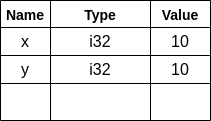
\includegraphics[width=0.3\textwidth]{img/memoria_2.png}
      \caption{Esquema de la memoria tras ejecutar dos asignaciones de números i32}
      \label{fig_memoria_2}
   \end{center}
\end{figure}

Este mecanismo de copia del valor en la nueva variable sucede siempre que los tipos implicados sean tipos primitivos y también con arrays y con tuplas de tipos primitivos. 

Observe, en cambio, el comportamiento cuando se hace un programa similar al anterior, pero en el que las variables son vectores:

\vspace{0.7em}
\begin{Codigo}
fn main() {
   let v = vec![10, 20];
   let w = x;
   println!("{:?}", w); // Imprime 10
   println!("{:?}", v); // ERROR, x no existe
}
\end{Codigo}

El programa anterior crea una variable \textit{v} de tipo \textit{Vec<i32>} y asigna valor a sus componentes. A continuación, crea una variable \textit{w} y le asigna el valor de \textit{v}. En asignaciones de este tipo, los vectores funcionan de manera diferente que los tipos primitivos (vea el esquema de la Figura \ref{fig_memoria_3}). 

Cuando se crea la variable \textit{w} y se le asigna el valor de \textit{v}, no se copia el valor de las componentes de \textit{v} en la nueva variable, lo que se asocia con la variable \textit{w} es la posición de memoria donde están guardadas las componentes del vector. En otros lenguajes, por ejemplo Java, a partir de ese momento habría dos variables en memoria, \textit{v} e \textit{w}, apuntando a la misma posición de memoria; se dice que Java \textit{asigna por referencia}, no por valor. En Rust, el funcionamiento es diferente: la variable \textit{w} se queda apuntando al valor, esto es, a la posición de memoria donde se guardan las componentes del vector, mientras que la variable \textit{v} queda inaccesible. Se dice que el valor de las componentes del vector se ha \textit{movido} de la variable \textit{v} a la variable \textit{w} o que la \textit{propiedad} del valor ha pasado de \textit{v} a \textit{w}.

La Figura \ref{fig_memoria_3} esquematiza este proceso. En la parte izquierda de la figura se muestra la situación tras la creación de la variable \textit{v}: se guarda la variable \textit{v} asociada a la posición de memoria en la que están almacenadas las componentes del vector, por ejemplo, la posición 5000. La parte derecha de la misma figura muestra la situación tras asignar a la variable \textit{w} el valor de la variable \textit{v}: la variable \textit{v} deja de existir y la propiedad del valor pasa a la variable \textit{w}\footnote{En realidad, la forma de asignar la memoria de un vector en Rust es un poco más compleja de lo que se esquematiza en la Figura \ref{fig_memoria_3}, pero a los efectos de la explicación del concepto de propiedad se ha considerado conveniente simplificarlo como se ha hecho.}.

\begin{figure}[htb]
   \begin{center}
      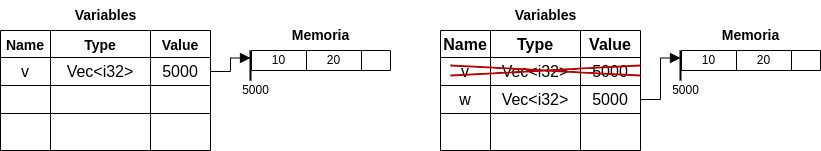
\includegraphics[width=\textwidth]{img/memoria_3.png}
      \caption{Izquierda: esquema de la memoria tras crear la variable \textit{v} del tipo \textit{Vec<i32>}. Derecha: esquema de la memoria tras asignar a la variable \textit{w} el valor de la variable \textit{v}}
      \label{fig_memoria_3}
   \end{center}
\end{figure}

En programación, se entiende por \textit{ámbito} de una variable (en inglés \textit{scope}) la parte del programa en la que dicha variable es accesible. En Rust, el ámbito de una variable lo determina el bloque en el que se crea la variable. Los bloques están delimitados entre dos llaves. Por ejemplo, en el siguiente código, la variable \textit{x} existe durante toda la extensión de la función \textit{main()}; en cambio, la variable \textit{y} solo existe dentro del bloque en el que se ha creado y cuando se intenta imprimir fuera de ese bloque, se produce un error.

\vspace{0.7em}
\begin{Codigo}
fn main() {
   let x= 10;
   {
      let y = 20;
   }
   println!("{:?}", x); // Imprime 10
   println!("{:?}", y); // ERROR, y no existe
}
\end{Codigo}

Las reglas por las que se rige el concepto de la \textit{propiedad de los valores} en Rust son las siguientes:

\begin{itemize}
   \item Cada valor tiene un propietario.
   \item En todo momento, cada valor tiene un solo propietario.
   \item Si se termina el ámbito del propietario, se destruyen el valor y el propietario.
\end{itemize}

Los tipos de datos que no están afectados por el concepto de propiedad se dice que se rigen por una semántica \textit{Copy}, mientras que los tipos que sí están afectados por el concepto de propiedad se dice que funcionan con semántica \textit{Move}.

\section{Referencias}
\noindent Es posible tomar prestada la propiedad de un valor utilizando una referencia al mismo. El compilador de Rust se encarga de comprobar que ninguna referencia sobreviva más allá que el valor al que apunta.

Hay dos tipos de referencias:

\begin{itemize}
   \item \textbf{Referencias inmutables (\&):} permiten utilizar el valor al que apuntan, pero no permiten modificarlo. Pueden existir al mismo tiempo varias referencias inmutables a un mismo valor en memoria.
   \item \textbf{Referencias mutables (\&mut):} permiten utilizar el valor al que apuntan y permiten también su modificación. Solo puede existir una referencia mutable a un valor en cada momento. Si durante la ejecución de un programa existe una referencia mutable a un valor en memoria, no pueden existir simultáneamente otras referencias al mismo valor, ni mutables ni inmutables.
\end{itemize}

Se denomina \textit{desreferenciar} a obtener el valor al que apunta una referencia. En muchas situaciones, Rust desreferencia directamente. Por ejemplo, si ejecuta el siguiente código, el valor que se imprime en pantalla es el valor al que apunta la referencia, no la referencia en sí misma:

\vspace{0.7em}
\begin{Codigo}
fn main() {
   let x = 32.6;
   let ref_x = &x;
   println!("{}", ref_x); // Imprime 32.6
}
\end{Codigo}

Hay ocasiones, no obstante, en que es necesario forzar la desreferenciación explícitamente. Para ello, se usa el operador $*$ (asterisco) colocado delante de la referencia, como se hace en el siguiente ejemplo:

\vspace{0.7em}
\begin{Codigo}
fn main() {
   let mut v = vec![10, 20, 30];
   for num in &mut v {
      if *num > 20 {
         *num = 40;
      }
   }
   println!("{:?}", v); // [10, 20, 40]
}
\end{Codigo}

Si se quiere imprimir la dirección de memoria a la que apunta una referencia, hay que utilizar la especificación de formato \textit{{:p}}:

\vspace{0.7em}
\begin{Codigo}
fn main() {
   let x = 32.6;
   let ref_x = &x;
   println!("{}", ref_x); // Imprime 32.6
   println!("{:p}", ref_x); // Imprime 0x7fff189f4bb8
}
\end{Codigo}



% -----------------------------------------------------------


%\input{apendices}

\pagestyle{empty}
\bibliography{../../Mibiblioteca.bib}


\end{document}

